%=======================================================================
% English edition preamble — RetNet-0.5B Technical Report
% Build: xelatex twice from docs/latex/en/
% Referenced by the `0p5b` configuration in mktex.py.
%=======================================================================
\documentclass[11pt,openany]{article}

% Latin text fonts
\usepackage{fontspec}
\setmainfont{Times New Roman}[Ligatures=TeX]
\setsansfont{Microsoft YaHei}
\setmonofont{Consolas}[Scale=0.86]

% CJK fallback.  The English edition is written in English throughout; the
% fallback exists for the repository paths and code comments that are part of
% the evidence, not for prose.
\usepackage{xeCJK}
\setCJKmainfont{SimSun}[BoldFont=SimHei,ItalicFont=KaiTi]
\setCJKmonofont{FangSong}
\xeCJKsetup{CJKmath=false}

% =====================================================================
%  preamble-common.tex
%  Shared preamble for the RetNet-272M technical report (Chinese and
%  English editions).  Build with XeLaTeX.
%
%  Typographic convention (deliberately plain, single column, as in a
%  conventional technical report):
%    * serif body text, no coloured display headings
%    * numbered tables and figures, each with a caption
%    * remarks set as an indented, labelled passage rather than a
%      coloured box
% =====================================================================

\usepackage{amsmath}
\usepackage{amssymb}
\usepackage{bm}

% ---------- layout ---------------------------------------------------
\usepackage[a4paper,top=2.5cm,bottom=2.5cm,left=2.4cm,right=2.4cm]{geometry}
\usepackage{fancyhdr}
\usepackage{titlesec}
\usepackage{enumitem}
\usepackage{booktabs}
\usepackage{array}
\usepackage{tabularx}
% A table taller than a page must be able to break across pages: an unbreakable
% `tabular` that large is shipped out past the paper edge (Overfull \vbox), and
% the part below the edge is what the reader loses.  `longtable` is used only
% for such tables (see mktex.render_table).
\usepackage{longtable}
\usepackage{ragged2e}
\usepackage{xcolor}
\usepackage{caption}
\usepackage{graphicx}

% ---------- code -----------------------------------------------------
\usepackage{listings}
\usepackage{newunicodechar}

% ---------- references ----------------------------------------------
\usepackage[hidelinks,bookmarksnumbered]{hyperref}
\usepackage{bookmark}

% ---------- colours (used sparingly: code and rules only) ------------
\definecolor{codebg}{RGB}{248,248,249}
\definecolor{codeframe}{RGB}{216,220,225}
\definecolor{codecomment}{RGB}{104,124,108}
\definecolor{codekeyword}{RGB}{0,80,150}
\definecolor{codestring}{RGB}{160,60,40}
\definecolor{rulecol}{RGB}{178,182,188}
\definecolor{headrule}{RGB}{40,48,60}

% ---------- spacing --------------------------------------------------
\linespread{1.04}
\setlength{\parskip}{0.30em}
\setlength{\parindent}{0pt}
\setlength{\abovedisplayskip}{6pt}
\setlength{\belowdisplayskip}{6pt}
\setlength{\abovedisplayshortskip}{4pt}
\setlength{\belowdisplayshortskip}{4pt}

% Mixed CJK / monospace prose has few hyphenation opportunities; give TeX
% more room to stretch instead of leaving overfull boxes.
\tolerance=3000
\emergencystretch=3em
\hyphenpenalty=50
\hbadness=10000

% ---------- headings: plain, black, not coloured ---------------------
\titleformat{\section}
  {\normalfont\large\bfseries}{\thesection}{0.7em}{}
\titleformat{\subsection}
  {\normalfont\normalsize\bfseries}{\thesubsection}{0.7em}{}
\titleformat{\subsubsection}
  {\normalfont\normalsize\itshape}{\thesubsubsection}{0.7em}{}
\titlespacing*{\section}{0pt}{1.5em}{0.55em}
\titlespacing*{\subsection}{0pt}{1.05em}{0.40em}
\titlespacing*{\subsubsection}{0pt}{0.85em}{0.30em}

% ---------- header / footer ------------------------------------------
\pagestyle{fancy}
\fancyhf{}
\renewcommand{\headrulewidth}{0pt}
\renewcommand{\footrulewidth}{0pt}
\fancyfoot[C]{\small\thepage}

% ---------- tables and figures ---------------------------------------
\renewcommand{\arraystretch}{1.18}
\setlength{\tabcolsep}{5pt}
\captionsetup{
  font=small,
  labelfont=bf,
  labelsep=period,
  justification=raggedright,
  singlelinecheck=false,
  skip=5pt,
}
\captionsetup[table]{position=top}
\captionsetup[figure]{position=bottom}

% A numbered table with its caption above, as in the reference report.
\newenvironment{reporttable}[1]
  {\begin{center}\small\captionof{table}{#1}}
  {\end{center}}
\newcommand{\tabnote}[1]{\par\vspace{2pt}{\footnotesize #1}}

% ---------- lists ----------------------------------------------------
\setlist[itemize]{topsep=0.25em,itemsep=0.12em,parsep=0.08em,leftmargin=1.5em}
\setlist[enumerate]{topsep=0.25em,itemsep=0.12em,parsep=0.08em,leftmargin=1.8em}

% ---------- inline code ----------------------------------------------
\newcommand{\code}[1]{\texttt{\small #1}}
\newcommand{\file}[1]{\texttt{\small #1}}

% ---------- code listings --------------------------------------------
\lstdefinestyle{report}{
  backgroundcolor=\color{codebg},
  basicstyle=\ttfamily\fontsize{8.1}{9.6}\selectfont,
  commentstyle=\color{codecomment}\itshape,
  keywordstyle=\color{codekeyword}\bfseries,
  stringstyle=\color{codestring},
  frame=single,
  rulecolor=\color{codeframe},
  framesep=5pt,
  framexleftmargin=5pt,
  xleftmargin=5pt,
  breaklines=true,
  breakatwhitespace=false,
  breakindent=1.2em,
  columns=fullflexible,
  keepspaces=true,
  showstringspaces=false,
  tabsize=4,
  aboveskip=0.6em,
  belowskip=0.6em,
  upquote=true,
  extendedchars=true,
  inputencoding=utf8,
  escapechar=|,
  texcl=false,
  literate=%
    {→}{{$\rightarrow$}}1
    {←}{{$\leftarrow$}}1
    {×}{{$\times$}}1
    {÷}{{$\div$}}1
    {≈}{{$\approx$}}1
    {≤}{{$\leq$}}1
    {≥}{{$\geq$}}1
    {≠}{{$\neq$}}1
    {µ}{{$\mu$}}1
    {γ}{{$\gamma$}}1
    {Δ}{{$\Delta$}}1
    {σ}{{$\sigma$}}1
    {τ}{{$\tau$}}1
    {Σ}{{$\Sigma$}}1
    {√}{{$\surd$}}1
    {·}{{$\cdot$}}1
    {−}{{$-$}}1
    {∈}{{$\in$}}1
    {±}{{$\pm$}}1
    {∞}{{$\infty$}}1
    {❌}{{$\times$}}1
    {✅}{{$\checkmark$}}1
    {⚠}{{!}}1
}
\lstset{style=report}

% `listings` ships no PowerShell dialect; define just enough to colour it.
\lstdefinelanguage{PowerShell}{
  morekeywords={if,else,elseif,foreach,for,while,function,param,return,
    try,catch,finally,switch,break,continue,throw,in,not,and,or},
  sensitive=false,
  morecomment=[l]{\#},
  morestring=[b]",
  morestring=[b]',
}
\lstdefinelanguage{text}{}

% ---------- remarks --------------------------------------------------
% The source uses block quotes for asides.  They are set as an indented
% passage introduced by "Note." rather than as a coloured box.
\newenvironment{notebox}
  {\par\vspace{0.35em}%
   \begin{list}{}{%
     \setlength{\leftmargin}{1.5em}\setlength{\rightmargin}{0.4em}%
     \setlength{\topsep}{0pt}\setlength{\parskip}{0.25em}%
     \setlength{\parsep}{0.25em}\setlength{\itemsep}{0pt}%
     \setlength{\listparindent}{0pt}}%
   \item\relax\textbf{Note.}\ \ignorespaces}
  {\end{list}\vspace{0.15em}}

% ---------- rule -----------------------------------------------------
\newcommand{\reportrule}{\par\vspace{0.5em}{\color{rulecol}\hrule height 0.4pt}\vspace{0.7em}\par}

% ---------- appendices -----------------------------------------------
% The source writes the appendix titles with their letter already in the
% text ("Appendix A: Reproduction"), so the appendix section counter prints
% the letter and the *headings* of the back matter use a second counter that
% renumbers (Reference Reliability Note, References).
\newcounter{backmatter}
\newcommand{\startappendix}{%
  \clearpage
  \setcounter{section}{0}%
  \setcounter{backmatter}{0}%
  \renewcommand{\thesection}{\Alph{section}.}%
  % subsections are numbered against the appendix letter, so pin the format
  % explicitly: leaving \thesubsection as \thesection.\arabic{subsection}
  % would print `B..1' because \thesection already ends in a period.
  \renewcommand{\thesubsection}{\Alph{section}.\arabic{subsection}}%
}
\newcommand{\backmattersection}[1]{%
  \refstepcounter{backmatter}%
  \section*{\arabic{backmatter}.\quad #1}%
  \addcontentsline{toc}{section}{\protect\numberline{\arabic{backmatter}.}#1}%
}


\hypersetup{
  pdftitle  = {RetNet-0.5B: Training a 504M-Parameter Retentive Network to Production, and Why Width Growth Never Unlocked},
  pdfauthor = {RetNet Project},
  pdfsubject= {Retentive Networks / Gated Linear Attention / Training Engineering / Serving},
  pdfkeywords={RetNet, GLA, chunkwise, torch.compile, 8-bit AdamW, 0.5B, single-node training},
}

\fancyhead[L]{\small\itshape RetNet-0.5B Technical Report}
\fancyhead[R]{\small\thepage}
\fancyfoot[C]{}

\begin{document}


%=======================================================================
% English edition title block and abstract -- RetNet-0.5B Technical Report
% Inserted before the body; the body comes from en_supplement.tex
% The title must match the H1 of docs/26_RetNet-0.5B_技术报告.md, and the
% abstract is a full translation of that file's `## 摘要`.
%=======================================================================
\thispagestyle{empty}

\begin{center}
\vspace*{2.6cm}

{\LARGE\bfseries RetNet-0.5B: Training a 504M-Parameter\\[0.25em] Retentive Network to Production}

\vspace{0.45cm}

{\large\bfseries and Why Width Growth Never Unlocked}

\vspace{0.7cm}

{\normalsize RetNet Project}

\vspace{0.25cm}

{\small\itshape 2026-10-13}

\vspace{1.5cm}

{% the caption of Table 1 belongs to the cover block of the source report
\small\textbf{Table 1.} Model summary (provenance per section of the body)}

\vspace{0.5em}

\begin{minipage}{0.94\textwidth}
\centering\small
\begin{tabular}{@{}rl@{}}
\toprule
Model & 504.18M parameters (504{,}179{,}896), 20 layers, width 1408, 22 heads \\
Training & three legs of one epoch; 1{,}656{,}209{,}408 tokens actually consumed \\
Hardware & RTX 3090 24\,GB / RTX PRO 6000 96\,GB / RTX 3070 8\,GB \\
Data & \code{chat\_pack\_v13}, 552{,}330{,}489 token slots, 2048-token context \\
Result & validation loss 2.6358 $\rightarrow$ 1.9459; 78 of the 82 growth affine tensors are bitwise zero \\
\bottomrule
\end{tabular}
\end{minipage}

\vfill

{\small\itshape This is the English edition; the Chinese edition is typeset as a
separate document from the same Markdown source.}

\vspace{1.0cm}
\end{center}

\clearpage

%-----------------------------------------------------------------------
% Abstract
%-----------------------------------------------------------------------
\section*{Abstract}
\addcontentsline{toc}{section}{Abstract}

RetNet's linear recurrence makes the memory cost of long-sequence inference independent of
sequence length, but it also means that a model of the half-billion-parameter class can only be
pushed forward by one card's memory and one card's time budget; every design choice in this
project is governed by those two constraints. This report records the complete engineering facts
of one specific model, \code{checkpoints/retnet\_500m\_v15b\_ep3}, from initialisation to online
service: \textbf{504{,}179{,}896} parameters, 20 layers, \code{d\_model} 1408, 22 heads, trained
on the \textbf{552{,}330{,}489} token slots of \code{data\_cache/chat\_pack\_v13} in \textbf{three
legs} (ep1 on an RTX 3090 24\,GB, ep2/ep3 on an RTX PRO 6000 96\,GB, leg by leg, no multi-GPU
parallelism), consuming \textbf{1{,}656{,}209{,}408} tokens in total (\textbf{3.28496} tokens per
nominal parameter; the three token definitions and their differences are in \S4.1), with
validation loss falling from \textbf{2.6358} to \textbf{1.9459}. The same weights switch between
three mathematically equivalent computation forms --- parallel, chunkwise and recurrent --- with
chunkwise used for training, parallel for prefill and recurrent for per-token decoding.

Three classes of engineering finding are worth recording separately. Of a 575\,ms step, 61.6\% is
GEMM and 3.8--4.3\% is removable structural redundancy. \textbf{Four classes of defect that raise
no error} (a checkpoint overriding the command-line batch size, the scheduler not resuming when
\code{optimizer.pt} is missing, the dead \code{--eval\_batches} field being silently ignored, the
throughput field using \code{max\_steps} as its numerator, and an equivalence test that used the
function under test as its own reference) each have reproducible log evidence. And one structural
measurement, re-checked by the project's verifier: of the 82 affine tensors added by growth,
\textbf{78 are bitwise zero} (the 4 counterexamples sit in L18/L19), so \textbf{67.08\%} of the
checkpoint's weight elements are exactly zero, with \code{gamma\_new = 0} self-locking as the
mechanism (\S2.4). That count is verified, but \textbf{no backward pass was run, so ``non-zero''
is not the same as ``trainable''}.

Evaluation and serving results are in \S5 and \S6; the model is served at
\href{https://your-demo-host.example/play/}{your-demo-host.example/play/}.

\clearpage

%-----------------------------------------------------------------------
% Contents
%-----------------------------------------------------------------------
\renewcommand{\contentsname}{Contents}
\tableofcontents

\clearpage


%=======================================================================
% RetNet-0.5B -- English edition body (full translation)
%
% The Chinese Markdown source is Chinese-only, so this file *is* the English
% edition: every section mirrors the Chinese edition section for section, and
% every number is taken from the Chinese final text (not from memory).  Table
% captions are attached by mktex.py from SUPPLEMENT_TABLE_HEADERS_05B, so a new
% table must have its header row registered there.
%=======================================================================

\section{Introduction}

This chapter states two things: what the constraints are, and why this report gives negative
results the same standing as positive ones.

The constraint is one card: an 8\,GB RTX 3070, a 24\,GB RTX 3090, a 96\,GB RTX PRO 6000. Every
increase in parameter count converts directly into memory and wall clock, and wall clock converts
into renminbi (unit prices in \S4.5). This is not an environment where the compute is ample and
only the hyper-parameters are missing: on the 24\,GB line the training-time memory margin is only
1{,}346\,MiB (23{,}230 / 24{,}576\,MiB), and on the 8\,GB line the 0.5B model has 517\,MiB of
margin. Batch size, precision, optimizer and gradient checkpointing therefore offer no room to
pick the optimum --- only ``fits'' or ``does not fit''.

RetNet (retentive network) replaces attention with a fixed geometric decay, and so the same model
has three mathematically equivalent computation forms: the parallel form trains well but its
memory grows with the square of sequence length, the recurrent form has constant memory but can
only advance one token at a time, and the chunkwise form is the compromise. What this report
cares about is whether the three can be exchanged on one set of weights and whether they agree
numerically (\S2.3 and \S6.1).

This report \textbf{proposes no new architecture}. It records one specific model: initialised
from scratch (via a function-preserving width growth), trained \emph{leg by leg} on an RTX 3090
and an RTX PRO 6000 for about 16.79 GPU-hours (each leg on its own card, no multi-GPU
parallelism), measured on a 1{,}020-item benchmark, and served publicly over a streaming
interface. It is worth writing down for three reasons. First, every performance number points at
a concrete file and field, including the estimates that were later refuted. Second,
\textbf{negative results get the same space as positive ones} (\S3.5, Appendix C): this project
does not distinguish between ``a few lines changed and it got faster'' and ``a few lines changed
and nothing happened''. Third, the report records four classes of \textbf{defects that raise no
error} (\S3.4), all of one family: the log looks normal, the numbers look plausible, and they are
wrong only under specific conditions.

\section{Architecture}

This chapter answers ``what does this model look like'', including the two departures from the
original RetNet paper and the measured evidence that one of them did not take effect in this
generation.

\subsection{Retention}

The original RetNet retention layer weights history by a per-head geometric decay $\gamma_h$.
The parallel form is

\[
\mathrm{Ret}(X)=\big(QK^{\top}\odot D\big)V,\qquad D_{ij}=\gamma_h^{\,i-j}\,[\,i\ge j\,],
\]

and the recurrent form writes the same thing as a state recurrence whose size is independent of
sequence length:

\[
S_n=\gamma_h\,S_{n-1}+k_n v_n^{\top},\qquad o_n=q_n^{\top}S_n .
\]

$\gamma_h$ is the knob for ``how long does this head remember'': $\gamma_h\to1$ means almost no
forgetting, $\gamma_h\to0$ means only the current token. The original paper sets
$\gamma_h=1-2^{-5-h}$, i.e. geometrically decreasing with the head index.

\subsection{The Learned Per-Head Decay Gate}

This implementation turns $\gamma$ from a fixed formula into a learned parameter (gated linear
attention, GLA): \code{retnet\_hf}\linebreak[0]\code{/modeling}\linebreak[0]\code{\_retnet}\linebreak[0]\code{.py:98-103} initialises it with $1-2^{-5-h}$ and,
when \code{use}\linebreak[0]\code{\_gla=true}, registers it as an \code{nn.Parameter} instead of a buffer. The
parameter \textbf{is $\gamma$, not $\log\gamma$}, so nothing in the parameterisation keeps it in
range and training can push it above 1 or to 0.

That leaves two boundaries that have to be handled explicitly. First, $\gamma$ must be stored in
fp32: bf16 has only 7 mantissa bits, so the ulp near 1.0 is about $2^{-8}$ and the decays of
neighbouring heads collapse onto the same value. This model's \code{config.json} has \code{dtype}
\code{float32} (the file has no \code{torch\_dtype} key), and every tensor read out of the weight
file is \code{F32}; the 440 measured $\gamma$ values run from a minimum of 0.1999 to a maximum of
0.9985. Second, each of the two ways to write the decay table breaks at one end of $\gamma$: the
factorised $\gamma^{i}\cdot\gamma^{-j}$ overflows fp32 as soon as $\gamma^{-255}$ is needed, and
the naive $\gamma^{\delta}$ is invalid for $\gamma>1$. \code{retnet\_hf}\linebreak[0]\code{/retention}\linebreak[0]\code{\_fast}\linebreak[0]\code{.py:51-92}
therefore always goes through log space, $\exp(\log\gamma\cdot\delta)$, with $\gamma$ clamped to a
positive floor so that $\exp(\log\gamma\cdot 0)=1$ at $\gamma=0$, matching the reference
implementation's $0^0=1$ (\code{retention}\linebreak[0]\code{\_fast}\linebreak[0]\code{.py:75-80}).

The gradient path corresponds one-to-one with the three places $\gamma$ appears: the parallel
$\gamma^{i-j}$, the four chunkwise tables
\code{inner\_mask}/\code{cross\_decay}/\code{value\_decay}/\code{chunk\_decay}, and the recurrent
$\gamma\cdot S_{n-1}$. $\gamma$ is a one-dimensional parameter, so the backward pass has to reduce
over the batch, sequence and chunk dimensions; that step is a line item of its own in the compute
ledger (\code{docs/25:30}, about 12\,GiB per step and about 7\,ms).

The measured $\gamma$ values of this model
(\code{checkpoints}\linebreak[0]\code{/retnet}\linebreak[0]\code{\_500m\_v15b}\linebreak[0]\code{\_ep3/model}\linebreak[0]\code{.safetensors}, the key \code{blocks.*.msr}\linebreak[0]\code{.gamma},
20 layers $\times$ 22 heads = 440 numbers) are: minimum \textbf{0.1999}, maximum \textbf{0.9985},
mean \textbf{0.6997}, and \textbf{no head exceeds 1}. The first 16 heads of layer 3 are
individually different (0.429 / 0.867 / 0.846 / 0.988 / \dots), while the last 6 heads equal the
same constant \textbf{0.5430} in \textbf{all 20 layers}; heads 12--15 are likewise 0.4462 in most
layers. The same constant repeating across layers is not a coincidence: AdamW's \textbf{decoupled
weight decay} keeps shrinking a parameter even when its gradient is zero,

\[
\gamma_{t+1}=\gamma_t\cdot\exp(-\eta_t\,w),
\]

where $\eta_t$ is that step's learning rate and $w$ is \code{weight}\linebreak[0]\code{\_decay}. Integrating the
step-by-step \code{learning}\linebreak[0]\code{\_rate} of the three \code{trainer}\linebreak[0]\code{\_state.json} files gives
$\sum_t\eta_t=6.1078$; multiplied by $w=0.1$ this predicts
$\gamma_{\text{pred}}=\gamma_{\text{init}}\cdot\exp(-0.6108)=0.5429$, against a measured
\textbf{0.5430} --- a difference of 0.02\%. The accurate statement about heads 16--21 is therefore
that they \textbf{never received a gradient, but were pushed down by about 45.7\% by weight
decay}; the 0.4462 of heads 12--15 needs a further $\sum_t\eta_t\approx1.96$ of the same decay to
explain (a \emph{derivation}, corresponding to training that continued after those heads had been
cut off by zero weights). Both are consequences that were verified, not hypotheses, and they
corroborate the measured structure of \S2.4.

\subsection{Three Computation Forms and the Closed-Form Chunkwise Scan}

The reference chunkwise form is a per-chunk loop: four matmuls per chunk plus a small state
recurrence. The batched formulation in \code{retnet\_hf}\linebreak[0]\code{/retention}\linebreak[0]\code{\_fast.py} compresses that into
three matmuls, by observing that the inter-chunk decay $d=\gamma^{C}$ is constant throughout the
loop, so the state before chunk $i$ has a closed form:

\[
S_{\text{prev}}[i]=d^{i}S_0+\sum_{j<i}d^{\,i-1-j}U_j,\qquad U_j=k_j^{\top}\big(v_j\odot\gamma^{\,C-1-\cdot}\big),
\]

which is a single batched matmul against the lower-triangular matrix
$T_{i,j}=d^{\,i-1-j}\,[\,i-1-j\ge0\,]$, i.e. $S_{\text{all}}=T\,U$. The difference from a
log-depth (Hillis--Steele) scan is that $T$ has only $H\cdot(nc+1)\cdot nc$ elements (5{,}984
fp32 values when $nc=16$ and $H=22$) and materialises no extra large tensor, whereas a log-depth
scan has to materialise a tensor on the order of $[B,H,nc,kd,vd]$ every round
(\code{retention}\linebreak[0]\code{\_fast}\linebreak[0]\code{.py:140-147} records that trade-off). Every exponent in the closed form is
non-negative, so there is no $\gamma^{-j}$ overflow: however small $\gamma$ is, it only
underflows to 0, which means history has been forgotten.

The three paths are selected by \code{RETNET\_FAST}\linebreak[0]\code{\_CHUNKWISE=}\linebreak[0]\code{1} and \code{mode}, and their
numerical agreement is given by tests and probes: chunkwise versus recurrent differ by
$1.326\times10^{-4}$ relative, chunkwise versus parallel by up to 3.395
(\code{scripts/grow}\linebreak[0]\code{\_500m}\linebreak[0]\code{.py:37-39}, on the short sequences used by the growth check). In other
words, ``mathematically equivalent'' means here that chunkwise and recurrent agree at the noise
floor, while \textbf{the parallel path is not bitwise equivalent at the 0.5B scale} (\S6.1).

\begin{center}\small
\captionof{table}{Purpose and per-step cost of the three computation forms}
\begin{tabular}{@{}>{\RaggedRight\arraybackslash}p{0.13\textwidth}>{\RaggedRight\arraybackslash}p{0.28\textwidth}>{\RaggedRight\arraybackslash}p{0.19\textwidth}>{\RaggedRight\arraybackslash}p{0.32\textwidth}@{}}
\toprule
\textbf{Form} & \textbf{Used for} & \textbf{Where} & \textbf{Per-step cost structure} \\
\midrule
parallel & prefill, short-sequence checks & \code{modeling}\linebreak[0]\code{\_retnet}\linebreak[0]\code{.py:180-185} & score matrix of size $L\times L$; memory grows with the square of sequence length \\
chunkwise & training (\code{mode=chunkwi}\linebreak[0]\code{se}, chunk 128) & \code{retention}\linebreak[0]\code{\_fast}\linebreak[0]\code{.py:95-180} & three batched matmuls plus an intra-chunk $C^2$ term \\
recurrent & per-token decoding, streaming state & \code{modeling}\linebreak[0]\code{\_retnet}\linebreak[0]\code{.py:197-211} & one outer-product update per token, constant state size \\
\bottomrule
\end{tabular}
\end{center}

\subsection{Growth Layer Norm --- and Why It Did Not Activate in This Model}

This model's 504M parameters were not initialised from scratch: they were \textbf{grown in width}
from a narrower checkpoint by putting the old weights into the top-left corner of the new
matrices, zero-filling the new rows and columns, and replacing LayerNorm with a two-part
\code{GrowthLayerN}\linebreak[0]\code{orm} (\code{retnet\_hf}\linebreak[0]\code{/modeling}\linebreak[0]\code{\_retnet}\linebreak[0]\code{.py:275-297}):

\[
\mathrm{LN}_{\text{grow}}(x)=\Big[\ \mathrm{LN}_{768}\big(x_{:768}\big),\ \ x_{768:}\odot\gamma_{\text{new}}+\beta_{\text{new}}\ \Big].
\]

The statistics of the old 768 coordinates depend only on those 768 coordinates, so widening does
not change the normalisation result; the new channels are controlled by an independent affine
pair initialised to zero, so growth is \textbf{strictly function-preserving at initialisation}.
In this model \code{growth\_old}\linebreak[0]\code{\_dim} is \textbf{768} against a \code{d\_model} of 1408, so every
normalisation has 640 new channels --- 41 places in all (40 layer norms,
\code{norm1}/\code{norm2} per layer, plus \code{final\_norm}).

The design intent of the growth script was that the new channels stay zero \textbf{until
unlocked} (\code{docs/08}\linebreak[0]\code{\_chunkwise}\linebreak[0]\code{\_growth}\linebreak[0]\code{\_research}\linebreak[0]\code{.md:57}). What was measured is that
\textbf{this batch of new channels was still locked in the ep3 checkpoint, and is bitwise zero}.

\begin{center}\small
\captionof{table}{Measured state of the growth layer norm's new dimensions}
\begin{tabular}{@{}>{\RaggedRight\arraybackslash}p{0.29\textwidth}>{\RaggedRight\arraybackslash}p{0.32\textwidth}>{\RaggedRight\arraybackslash}p{0.31\textwidth}@{}}
\toprule
\textbf{Check} & \textbf{Measured} & \textbf{Reading} \\
\midrule
82 \code{*.gamma\_new}/\code{*.beta\_new} tensors (41 places $\times$ 2) & \textbf{78 bitwise zero}; all 41 \code{gamma\_new} are zero, \code{beta\_new} has 4 counterexamples & every normalisation output is identically 0 beyond dimension 768 (counterexamples in the next row) \\
the 4 counterexamples: \code{blocks.\{18,19\}.}\linebreak[0]\code{norm\{1,2\}.}\linebreak[0]\code{beta\_new} & \textbf{256 non-zero} each, local index \code{[0,255]} $\rightarrow$ dims \code{[768,1023)}, range \textbf{$-0.1138$ \dots\ $+0.1490$} & those 4 \code{beta\_new} can leave zero because they belong to the inserted layers' (L18/L19) 1024-wide read side; \textbf{they are the strongest corroboration of the self-lock} --- \code{gamma\_new} in the same module is still identically zero \\
\code{embedding}\linebreak[0]\code{.weight[:, 7}\linebreak[0]\code{68:1408]} (20000 $\times$ 640) & \textbf{all zero} (12{,}800{,}000 elements) & the widened residual stream has no non-zero source at its input \\
new row/column blocks of the seven linear matrices in L0--L17 (\code{q/k/v/g}\linebreak[0]\code{\_proj}, \code{out\_proj}, \code{ffn.0/2}) & \textbf{all zero}; the whole layer's zero share is \textbf{70.2\%} & the widened rows and columns were never written \\
the zero regions of L18/L19 are \textbf{asymmetric} & zero share \textbf{51.5\%} per layer; the read side is dead on \code{[1024,1408)} (384 dims), the write-back to the residual is dead on \code{[768,1408)} (640 dims) & these two are the inserted layers (full-width insertion plus zero residual write-back, \code{scripts/grow}\linebreak[0]\code{\_272m}\linebreak[0]\code{.py:25,28}); their structure differs from the other 18 \\
weight elements exactly zero, whole checkpoint & \textbf{338{,}196{,}736 / 504{,}179{,}896 = 67.08\%} & non-zero elements: 165{,}983{,}160 (32.9\%) \\
\bottomrule
\end{tabular}
\end{center}

\begin{notebox}
One accompanying configuration fact: \code{growth\_old}\linebreak[0]\code{\_dim=768} in
\code{checkpoints}\linebreak[0]\code{/retnet}\linebreak[0]\code{\_500m}\linebreak[0]\code{/config.json} is \textbf{correct only for L0--L17}; L18/L19 are
inserted layers whose real cut points are \textbf{1024 (read side) / 768 (write-back side)}.
\end{notebox}

The mechanism can be stated completely, with no extra assumption: if the new input columns are
always zero and the normalisation clamps everything beyond dimension 768 to zero, then the
downstream partial derivative with respect to those dimensions is always zero, so the gradients
of those weights and of $\gamma_{\text{new}}/\beta_{\text{new}}$ are always zero, and they stay
at their growth-time zero --- a self-locking dead subspace. \textbf{That causal chain is a
mechanism derivation} (aligned with the code and the measurements); the verifier has signed off on
the two counts ``67.08\% of weights are exactly zero'' and ``78/82 tensors are zero'', so they may
be used in the abstract, but \textbf{this report ran no backward pass, so ``non-zero'' is not the
same as ``trainable''}, and the budget conclusions of \S4.6 and \S5.5 are not rewritten on the
strength of it.

On those measurements the non-zero elements number \textbf{165{,}983{,}160} (150{,}470{,}656 of
them in the 20 layers' seven linear matrices and 15{,}360{,}000 in the first 768 columns of the
embedding); if those zero elements really take no part in the computation, then the ``tokens per
non-zero parameter'' corresponding to the 1{,}656{,}209{,}408 tokens the three legs consumed is
\textbf{9.9782}, not the nominal \textbf{3.28496} (a change of denominator over the same tokens,
not a claim about trainable capacity --- see the qualification above).

\subsection{0.5B Configuration}

\begin{center}\small
\captionof{table}{Model configuration}
\begin{tabular}{@{}>{\RaggedRight\arraybackslash}p{0.24\textwidth}>{\RaggedRight\arraybackslash}p{0.24\textwidth}>{\RaggedRight\arraybackslash}p{0.24\textwidth}>{\RaggedRight\arraybackslash}p{0.20\textwidth}@{}}
\toprule
\textbf{Field} & \textbf{Value} & \textbf{Field} & \textbf{Value} \\
\midrule
\code{d\_model} & 1408 & \code{num\_layers} & 20 \\
\code{num\_heads} & 22 & \code{key\_dim} (exported) & 64 \\
\code{value\_dim} / \code{ffn\_dim} & 2816 / 2816 & \code{vocab\_size} & 20000 \\
\code{chunk\_size} & 128 & \code{mode} & \code{chunkwise} \\
\code{dropout} & 0.1 & \code{norm\_eps} & 1e-05 \\
\code{use\_gla} & true & \code{use\_growth}\linebreak[0]\code{\_ln} / \code{growth\_old}\linebreak[0]\code{\_dim} & true / 768 \\
\code{use\_swiglu} & \textbf{false} (FFN is Linear+GELU+Linear) & \code{tie\_weights} & true \\
\code{embed\_scale} & 27.712812921102035 ($=\sqrt{768}$) & \code{prompt\_loss}\linebreak[0]\code{\_weight} & 0.1 \\
\code{checkpoint}\linebreak[0]\code{\_layers} & $-1$ (all layers) & \code{dtype} & \code{float32} \\
\code{transformers}\linebreak[0]\code{\_version} & 4.57.6 & \code{model\_type} & \code{retnet\_hf} \\
\code{architecture}\linebreak[0]\code{s} & \code{RetNetForCau}\linebreak[0]\code{salLM} & parameters & 504{,}179{,}896 \\
sha256 (recomputed with \code{Get-FileHash} before delivery) & \code{dd7cdc90ae76}\linebreak[0]\code{c81c4c7134bb}\linebreak[0]\code{5e614455f924}\linebreak[0]\code{a8ffa51075c6}\linebreak[0]\code{646728cd290a}\linebreak[0]\code{3c53} & file size & 2{,}016{,}755{,}680 B \\
\bottomrule
\end{tabular}
\end{center}

\code{use}\linebreak[0]\code{\_swiglu=fal}\linebreak[0]\code{se} leaves the FFN with a single branch, so there is none of the SwiGLU
redundancy in which \code{norm2} is called twice (\code{docs}\linebreak[0]\code{/25:121-125});
\code{use\_growth}\linebreak[0]\code{\_ln=true, g}\linebreak[0]\code{rowth\_old}\linebreak[0]\code{\_dim=768} is the source of the 41 \code{cat}+slice pairs.

\section{General Infrastructures}

This chapter answers ``how does this stack run, how large can it run, where does a step's time go,
and what fails without reporting'', and it is the longest chapter of the report, because every
item in it comes from the real training path rather than from a micro-benchmark.

\subsection{Training Stack}

The entry point is \code{retnet\_hf}\linebreak[0]\code{/train.py} (406 lines), which wraps the HuggingFace
\code{Trainer} (transformers 4.57.6) into a task-configuration-driven script: \code{tasks/*.json}
describes one run, \code{run\_task.py} translates it into a command line, and
\code{scripts}\linebreak[0]\code{/linux/run}\linebreak[0]\code{\_train.sh} handles cloud start/stop, watchdog and finalisation. The
hyper-parameters that actually took effect are in Appendix A.

Four engineering decisions on this stack are worth stating separately:

\begin{enumerate}
  \item \textbf{\code{torch}\linebreak[0]\code{.compile} replaces \code{forward} in place, rather than wrapping the
        module in an \code{OptimizedMod}\linebreak[0]\code{ule}} (\code{train}\linebreak[0]\code{.py:327-357}): \code{state}\linebreak[0]\code{\_dict()}
        keys stay clean and the exported file loads normally through \code{from}\linebreak[0]\code{\_pretrained}.
  \item \textbf{The export is self-checked for its key names}: \code{verify}\linebreak[0]\code{\_export}
        (\code{train}\linebreak[0]\code{.py:61-88}) reads the safetensors header directly, and all three legs end
        their log with \code{[verify]} reporting 365 clean export keys (\code{v16\_ep2.out},
        \code{v17\_ep3.out}).
  \item \textbf{triton is checked explicitly before compiling}: inductor compiles lazily, so a
        missing triton does not raise at the \code{torch}\linebreak[0]\code{.compile()} call --- it silently falls
        back to eager (\code{train}\linebreak[0]\code{.py:313-325}).
  \item \textbf{An external control flag}: \code{logs/ctrl}\linebreak[0]\code{.txt}
        (\code{run}/\code{stop}/\code{next-checkpo}\linebreak[0]\code{int}/\code{save}) is read by a callback
        (\code{retnet\_hf}\linebreak[0]\code{/control.py}), so a shutdown can save a checkpoint and then let training
        return normally, instead of \code{taskkill} --- which returns rc=1 and triggers the
        automatic restart.
\end{enumerate}

\subsection{The Feasible Envelope of Memory and Batch Size}

The feasible configurations and measured peaks of the three real hardware lines are below; the
8\,GB numbers come from a 500M probe on a desktop 3070, the 24/96\,GB numbers from the sampling
files of the real runs.

\begin{center}\small
\captionof{table}{Feasible configurations and measured peaks on three devices}
\begin{tabular}{@{}>{\RaggedRight\arraybackslash}p{0.13\textwidth}>{\RaggedRight\arraybackslash}p{0.28\textwidth}>{\RaggedRight\arraybackslash}p{0.22\textwidth}>{\RaggedRight\arraybackslash}p{0.17\textwidth}>{\RaggedRight\arraybackslash}p{0.12\textwidth}@{}}
\toprule
\textbf{Device} & \textbf{Feasible configuration} & \textbf{Measured peak} & \textbf{Step time / throughput} & \textbf{Margin} \\
\midrule
RTX 3070 8\,GB & batch $1\times4$, \textbf{full gradient checkpointing}, 8-bit Adam, chunk 128 & 6.91\,GiB reserved (\code{logs/scale}\linebreak[0]\code{\_probe}\linebreak[0]\code{/results.txt} E3a, 1{,}891\,ms row; repeat 1{,}831\,ms) & 1{,}831--1{,}891\,ms per optimization step & \textbf{517\,MiB} (against 7{,}593\,MiB usable) \\
RTX 3090 24\,GB & batch $4\times1$, \textbf{checkpointing off}, 8-bit Adam, chunk 128 & 23{,}118\,MiB (\code{\_peak}\linebreak[0]\code{\_v15b*.txt}, max of 6{,}734 samples) / 23{,}230\,MiB (another segment, max of 1{,}289) & 0.6046\,s per step (11.3161\,h $\div$ 67{,}390) & \textbf{1{,}346\,MiB} \\
RTX PRO 6000 96\,GB & batch $16\times1$, checkpointing off, 8-bit Adam, chunk 128 & 77{,}685\,MiB (ep3) / 80{,}433\,MiB (ep2) & 0.5737\,s per step (ep3, whole leg amortised) & about 17--20\,GiB \\
\bottomrule
\end{tabular}
\end{center}

Each boundary has an explanation. \textbf{Gradient checkpointing is a hard requirement on 8\,GB}:
without it, the activations of 0.5B need about 7.2\,GiB, more than the whole usable card
(\code{docs}\linebreak[0]\code{/22:480-483}). \textbf{Turning it off is the largest single lever of this generation,
but the two lines start from different points}: the 500M probe on the 8\,GB line (full
checkpointing) is \textbf{1{,}831\,ms}, while the real 24\,GB path falls from \textbf{944\,ms to
510\,ms} (probe basis, 1.851$\times$, \code{docs}\linebreak[0]\code{/23:506-512}) --- 1{,}831 is the 8\,GB probe's
basis and cannot be used as the 24\,GB line's starting point. \textbf{8-bit Adam is a requirement,
not an optimization}: on the state ledger of $P\times10.004$\,B, 504.18M parameters occupy
\textbf{5.04\,GB $\approx$ 4.70\,GiB}, whereas fp32 AdamW ($P\times16.004$\,B) needs
\textbf{8.07\,GB $\approx$ 7.51\,GiB} --- a difference of \textbf{2.81\,GiB}, more than the whole
margin of the 8\,GB line (a derivation; the measured evidence is that ``batch 1 + accumulation
without 8-bit Adam'' goes into memory thrashing, \code{docs/23:602}). And
\textbf{\code{eval\_batch}\linebreak[0]\code{\_mult} must be 1}: taking the evaluation batch four times the training
batch triggers a recompile and pushes reserved memory to the wall; in one 8\,GB run the
evaluation overhead was 6.6\%, and it fell to 2.9\% at 1$\times$ (\code{train}\linebreak[0]\code{.py:188-195}). All
three legs use 1, so every evaluation covers all 833 validation rows; \textbf{the first evaluation
of a run pays for the compile warm-up} --- 90.86\,s for ep2's first, 23.08\,s for ep3's, and
9.53--9.60\,s afterwards.

In the table, ep2's peak (80{,}433\,MiB) is \textbf{higher} than ep3's (77{,}685\,MiB) although the
two configurations are identical. That is not a configuration difference but a sampling-window
difference: the peak is sampled every 5 seconds, and which checkpoint/evaluation transient a
sample catches depends on where the window falls. This has to be stated whenever a peak is
quoted.

\subsection{Composition of One Step}

\begin{figure}[htbp]
\centering
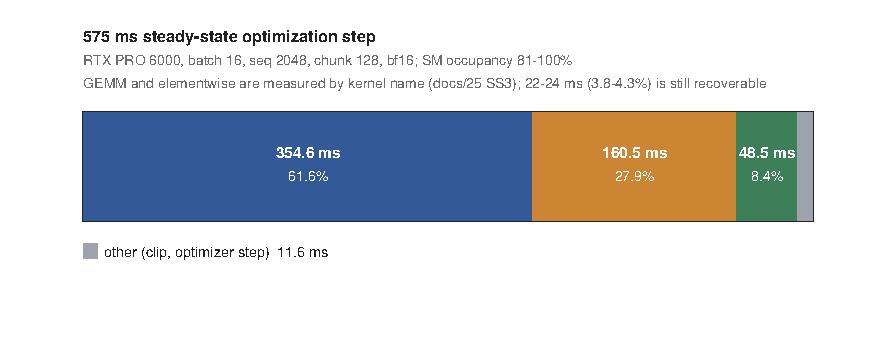
\includegraphics[width=\linewidth]{../figures/fig-0p5b-step}
\caption{Where one 575\,ms optimization step goes (RTX PRO 6000, batch 16, seq 2048, chunk 128, bf16). GEMM and the Triton kernels are bucketed by kernel name from a real profile; 22--24\,ms of the step is still recoverable.}
\label{fig:fig-0p5b-step}
\end{figure}

The decomposition below comes from \code{docs/25}, on the basis of a \textbf{575\,ms optimization
step at RTX PRO 6000 / batch 16 / seq 2048 / chunk 128 / bf16}: the GEMM, elementwise and
reduction rows are \emph{measured}, bucketed by kernel name from one real profile, while the byte
ledger is a \emph{derivation} from tensor shapes and read/write passes (that document reports
itself as overestimating by 2--3$\times$ on known ablations, so each item reads as an upper
bound).

\begin{center}\small
\captionof{table}{Composition of one optimization step}
\begin{tabular}{@{}>{\RaggedRight\arraybackslash}p{0.42\textwidth}>{\RaggedRight\arraybackslash}p{0.20\textwidth}>{\RaggedRight\arraybackslash}p{0.20\textwidth}@{}}
\toprule
\textbf{Category} & \textbf{Time} & \textbf{Share} \\
\midrule
GEMM (cuBLAS, forward and backward) & 354.6\,ms & 61.6\% \\
Triton elementwise kernels & 160.5\,ms & 27.9\% \\
Triton reduction kernels & 48.5\,ms & 8.4\% \\
other (clip, optimizer step, \dots) & 11.6\,ms & 2.0\% \\
\textbf{total} & \textbf{575\,ms} & 100\% \\
\bottomrule
\end{tabular}
\end{center}

The hardware state in the same window: SM occupancy 81--100\% (mean 93\%), memory bandwidth
53--71\%, power 480/600\,W, no throttling. The measured whole-leg throughput (57{,}111\,tok/s)
against this model's arithmetic intensity gives \textbf{MFU 45.8\%}
($57{,}111\times3.136$\,GFLOP/token $\div$ 391\,TFLOP/s), where 391\,TFLOP/s is the \emph{measured}
8192\textsuperscript{3} bf16 GEMM peak on that card rather than its nameplate figure.

The per-operator byte ledger comes to \textbf{about 274\,GiB per step} (range 150--300, depending
on how much inductor has fused), whose floor at the card's 1.79\,TB/s nameplate bandwidth is
164\,ms; the measured pointwise plus reduction total is 209\,ms, i.e. \textbf{1.41\,TB/s = 79\% of
nameplate} --- normal for pointwise kernels mixing broadcasts and transposes. \textbf{There is no
hidden 100\,ms free lunch in that ledger.}

\begin{center}\small
\captionof{table}{Recoverable step-time changes that were not landed}
\begin{tabular}{@{}>{\RaggedRight\arraybackslash}p{0.34\textwidth}>{\RaggedRight\arraybackslash}p{0.28\textwidth}>{\RaggedRight\arraybackslash}p{0.26\textwidth}@{}}
\toprule
\textbf{Change} & \textbf{Location} & \textbf{Recoverable} \\
\midrule
\code{rotate}\linebreak[0]\code{\_every\_two} without the \code{torch.stack} materialisation & \code{modeling}\linebreak[0]\code{\_retnet}\linebreak[0]\code{.py:72-76} & 8.3\,ms \\
\code{GrowthLayerN}\linebreak[0]\code{orm} fused (removing \code{cat} + slice) & \code{modeling}\linebreak[0]\code{\_retnet}\linebreak[0]\code{.py:294-297} & 8.5\,ms \\
\code{inner + cros}\linebreak[0]\code{s}'s separate add turned into \code{baddbmm} & \code{retention}\linebreak[0]\code{\_fast}\linebreak[0]\code{.py:179} & 6.2\,ms \\
\textbf{total} & & \textbf{22--24\,ms (3.8--4.3\% of one step)} \\
\bottomrule
\end{tabular}
\end{center}

The same document states two ``where the ledger was wrong'' corrections, both re-checked: the
claim that the decay matrix is a large $[B,H,T,T]$ tensor does not hold --- the real $T$ is only
23\,KiB --- and the claimed 8--10\% speed-up from removing \code{clone}/\code{slice}\linebreak[0]\code{\_backward}
does not hold either: counted operator by operator it is worth about 3.5\,ms (0.6\%).

\subsection{Defects That Raise No Error, in Four Classes by Consequence}

This section is the part of the report most worth reusing. The \textbf{five concrete defects}
that were actually hit during this generation's training and serving, with evidence left behind,
fall into \textbf{four classes by consequence}; what they share is that they \textbf{raise no
exception, look numerically plausible, and are wrong only under specific conditions} --- and each
one only revealed itself after it had been fixed. \textbf{This is not claimed to be an exhaustive
list.}

\begin{center}\small
\captionof{table}{The defects that raised no error, grouped by consequence}
\begin{tabular}{@{}>{\RaggedRight\arraybackslash}p{0.17\textwidth}>{\RaggedRight\arraybackslash}p{0.27\textwidth}>{\RaggedRight\arraybackslash}p{0.24\textwidth}>{\RaggedRight\arraybackslash}p{0.24\textwidth}@{}}
\toprule
\textbf{Class} & \textbf{Defect} & \textbf{Consequence} & \textbf{Evidence} \\
\midrule
(1) training numerics silently changed & \code{--resume} overridden by the checkpoint's \code{train\_batch}\linebreak[0]\code{\_size} (16 $\rightarrow$ 4) & the real batch disagrees with the configuration, and it self-locks & \code{transformers}\linebreak[0]\code{/trainer}\linebreak[0]\code{.py:2298}; \code{retnet\_hf}\linebreak[0]\code{/train.py:91} (definition) / \code{:394} (call); \code{logs}\linebreak[0]\code{/gpu-host}\linebreak[0]\code{\_20261013}\linebreak[0]\code{/linux/train}\linebreak[0]\code{\_20261012}\linebreak[0]\code{\_212943}\linebreak[0]\code{.log:43} \\
(1) same & a missing \code{optimizer.pt} also prevents \code{scheduler.pt} from loading, so the learning rate restarts from its peak & the LR curve is wrong and the loss rebound is misread as ``training broke'' & \code{transformers}\linebreak[0]\code{/trainer}\linebreak[0]\code{.py:3524} (\code{:3523} is the preceding assignment); \code{logs/resume}\linebreak[0]\code{\_B.out} \\
(2) configuration silently ignored & \code{--eval}\linebreak[0]\code{\_batches} is a dead field: declared and never read & the evaluation batch count on the command line is decoration; every evaluation runs the full set & \code{retnet\_hf}\linebreak[0]\code{/train}\linebreak[0]\code{.py:175} (its only occurrence in the file) \\
(3) metrics distorted & \code{train\_steps}\linebreak[0]\code{\_per}\linebreak[0]\code{\_second} $\equiv$ \code{max\_steps }\linebreak[0]\code{/ runtime} & segmented or resumed runs overstate throughput by up to 6.32$\times$ & \code{transformers}\linebreak[0]\code{/trainer}\linebreak[0]\code{.py:2823}; \code{trainer}\linebreak[0]\code{\_utils}\linebreak[0]\code{.py:389} (definition), \code{:411} (the division) \\
(4) a test spinning idle & the equivalence test's ``reference path'' was the function under test & that test can never discover this defect & \code{modeling}\linebreak[0]\code{\_retnet}\linebreak[0]\code{.py:215-217}; \code{tests/test}\linebreak[0]\code{\_fast}\linebreak[0]\code{\_chunkwise}\linebreak[0]\code{.py:31} \\
\bottomrule
\end{tabular}
\end{center}

\textbf{(1)-a \ Checkpoint overrides the command-line batch.} Symptom: the command line said
\code{--batch}\linebreak[0]\code{\_size 16}, but the run only used 30{,}177\,MiB and 51.2k\,tok/s, whereas a
same-architecture batch-16 probe needs 75.25\,GiB and runs at 57.1k--61.0k\,tok/s. Location: in
\code{Trainer}\linebreak[0]\code{.train()} HF overrides \code{self.\_train}\linebreak[0]\code{\_batch}\linebreak[0]\code{\_size} with
\code{state.train}\linebreak[0]\code{\_batch}\linebreak[0]\code{\_size} (\code{trainer}\linebreak[0]\code{.py:2298}), and the former is exactly what the
\code{DataLoader} is built with; the only trace is one WARNING line,
\code{per\_device}\linebreak[0]\code{\_train}\linebreak[0]\code{\_batch}\linebreak[0]\code{\_size: 16 (}\linebreak[0]\code{from args) !}\linebreak[0]\code{= 4 (from tr}\linebreak[0]\code{ainer\_state}\linebreak[0]\code{.json)}. A third-party
cross-check is the epoch field: \code{steps\_in}\linebreak[0]\code{\_epoch} = 269{,}561/4 = 67{,}390, and at the
observed step 70{,}180 the epoch read 1.04 ($=1+2{,}790/67{,}390$); with batch 16
(\code{steps\_in}\linebreak[0]\code{\_epoch} = 16{,}848) it should have read \textbf{4.17}. Fix:
\code{\_sync}\linebreak[0]\code{\_resume}\linebreak[0]\code{\_state()} (\code{retnet\_hf}\linebreak[0]\code{/train}\linebreak[0]\code{.py:91-157}) aligns those four fields before
training, prints \code{old -> new}, and leaves a \code{trainer}\linebreak[0]\code{\_state.json}\linebreak[0]\code{.orig} behind. Note that
this defect \textbf{self-locks}: each newly written checkpoint records 4
(\code{checkpoint-7}\linebreak[0]\code{0000/trainer}\linebreak[0]\code{\_state.json}'s \code{train\_batch}\linebreak[0]\code{\_size: 4}; that file is a cloud
artefact and was not re-checked locally), so without the fix every resume returns to 4. Local
reproduction: \code{logs/local}\linebreak[0]\code{\_resume}\linebreak[0]\code{\_test\_ep3}\linebreak[0]\code{.out} printed \code{train\_batch}\linebreak[0]\code{\_size 16 ->}\linebreak[0]\code{ 1}.
A methodological footnote: the function body existed before its call site and went uncalled for a
long time (\code{train}\linebreak[0]\code{.py:386-394}) --- ``guarding against this trap'' was once an empty promise.

\textbf{(1)-b \ A missing \code{optimizer.pt} also stops the scheduler from resuming.} Symptom:
after a resume, loss rebounded from 2.0009 to 2.13--2.39. Location: the actual condition line is
\code{if checkpoin}\linebreak[0]\code{t\_file}\linebreak[0]\code{\_exists and}\linebreak[0]\code{ os.path}\linebreak[0]\code{.isfile(..}\linebreak[0]\code{.SCHEDULER}\linebreak[0]\code{\_NAME)}
(\code{trainer}\linebreak[0]\code{.py:3524}; \code{:3523} is the preceding assignment), where the first term means
\code{optimizer.pt}; this round did not transfer the 1.11\,GB \code{optimizer.pt} to save time, so
\code{scheduler.pt} was present but never loaded and the LR warmed up again from step 0. Measured:
the previous leg's last step had \code{learning}\linebreak[0]\code{\_rate = 1}\linebreak[0]\code{.1000e-05} (the cosine floor) and the
resumed run's first segment had \code{1.0987e-04} ($\approx$ peak, 10$\times$); back-integrating
gives \code{last\_epoch} $\approx$ 2{,}790, exactly that segment's step count from its own start.
Fix: \code{\_sync}\linebreak[0]\code{\_resume}\linebreak[0]\code{\_state()} detects the absence and warns explicitly
(\code{train}\linebreak[0]\code{.py:153-157}); \code{logs/resume}\linebreak[0]\code{\_B.out} carries the same line. \textbf{This one turns
the impression ``training broke'' back into a known scheduler-state problem.}

\textbf{(2) \ Configuration silently ignored.} Symptom: the command line said
\code{--eval}\linebreak[0]\code{\_batches 40}, so evaluation appeared to run 40 batches. Location:
\code{retnet\_hf}\linebreak[0]\code{/train}\linebreak[0]\code{.py:175} declares the parameter (default 40) but \textbf{it is the only
occurrence in the whole file} and nothing ever reads it; every evaluation covers the entire
validation set (measured \code{eval}\linebreak[0]\code{\_samples}\linebreak[0]\code{\_per}\linebreak[0]\code{\_second} $\approx$ 87.2, 833 rows). Fix: either
wire it up or delete it --- \textbf{the current state is the worst of the three: the configuration
looks as if it works while being decoration.} (The \code{train.py:106} reference in a
\code{tasks/v15b}\linebreak[0]\code{\_500m\_24g}\linebreak[0]\code{.json} comment is stale; that line is blank. The real declaration is at
\code{:175}.)

\textbf{(3) \ The throughput field uses \code{max\_steps} as its numerator.} Symptom: within one
run the logged steps/second can be off by a multiple. Location:
\code{transformers}\linebreak[0]\code{/trainer}\linebreak[0]\code{.py:2819-282}\linebreak[0]\code{5} calls \code{speed}\linebreak[0]\code{\_metrics(..}\linebreak[0]\code{., num}\linebreak[0]\code{\_steps=self}\linebreak[0]\code{.state.max}\linebreak[0]\code{\_steps, ..}\linebreak[0]\code{.)}
at the end of training, and \code{speed}\linebreak[0]\code{\_metrics} (defined at \code{trainer}\linebreak[0]\code{\_utils}\linebreak[0]\code{.py:389}, doing
the division at \code{:411}) computes \code{num\_steps }\linebreak[0]\code{/ runtime}, so
\textbf{\code{train\_steps}\linebreak[0]\code{\_per}\linebreak[0]\code{\_second} $\equiv$ \code{max\_steps }\linebreak[0]\code{/ train}\linebreak[0]\code{\_runtime}}. The numeric
test passes 5 out of 5: \code{v15b\_real}\linebreak[0]\code{.out} reports 10.304 ($=$ 67{,}390 $\div$ 6{,}540.3172\,s),
\code{v15b\_resume}\linebreak[0]\code{.out} 1.971, ep2/ep3 1.678 / 1.743, and \code{v15c}\linebreak[0]\code{\_pro6000}\linebreak[0]\code{.out} 72.34. For runs
that stop early or resume in segments the field is necessarily wrong: seg1 actually ran 10{,}661
steps, i.e. a true 1.6300 steps/s (\textbf{reported 6.32$\times$ high}) and seg2 1.6633 steps/s
(1.185$\times$); ep2/ep3 ran every step and happened to be right --- \textbf{and ``happening to be
right'' is exactly what makes it dangerous.} Fix: every throughput number in \S4.5 is recomputed
from real steps and real tokens.

\textbf{(4) \ The equivalence test compares a function with itself.} Symptom: the equivalence test
for the batched chunkwise kernel reported ``bitwise identical'' for a long time. Location:
\code{modeling}\linebreak[0]\code{\_retnet}\linebreak[0]\code{.py:215-217} \textbf{forwards directly} to \code{chunkwise}\linebreak[0]\code{\_batched} when
\code{FAST}\linebreak[0]\code{\_CHUNKWISE=}\linebreak[0]\code{1}, and the training environment had that variable on, so the test's
``reference implementation'' was the function under test --- it never compared anything
(\code{tests/test}\linebreak[0]\code{\_fast}\linebreak[0]\code{\_chunkwise}\linebreak[0]\code{.py}'s \code{reference}\linebreak[0]\code{\_path} docstring records this). Fix: turn
the module-level switch off before taking the reference value, and compare relatively rather than
against the old absolute threshold of 1e-4, which judged a pile of correct results with
$10^{-7}$ relative error as non-equivalent. The same test has a second blind spot: the model-level
case passed under the old initialisation because \code{group\_norm}\linebreak[0]\code{.weight} was zeroed, making the
retention branch output identically zero, so both paths compared two all-zero contributions; only
with the weight set to 1 does a real comparison start (fp32 relative difference 8.6e-7,
\code{docs/22} \S0 item 18). \textbf{A check that cannot fail is not a check.}

\subsection{Negative Results}

This section lists the changes that were made but did not help --- or were slower --- each with its
measured numbers. They matter as much as the positive results: these experiments have essentially
exhausted this generation's optimization space, and what is left is ``bandwidth efficiency''
rather than ``a large lever not yet found''.

\begin{center}\small
\captionof{table}{Negative results}
\begin{tabular}{@{}>{\RaggedRight\arraybackslash}p{0.28\textwidth}>{\RaggedRight\arraybackslash}p{0.38\textwidth}>{\RaggedRight\arraybackslash}p{0.24\textwidth}@{}}
\toprule
\textbf{Item} & \textbf{Result} & \textbf{Evidence / basis} \\
\midrule
Layered gradient checkpointing (checkpointing only the first $K$ layers) & on the 500M probe with $K=16/20$: \textbf{2{,}793\,ms / 7.62\,GiB}, against \textbf{1{,}891\,ms / 6.91\,GiB} for checkpointing everything --- \textbf{slower and hungrier}, strictly dominated & 8\,GB line + 500M probe, \code{docs/23:591}; \code{logs/scale}\linebreak[0]\code{\_probe2/} \\
CPU activation offload (\code{save\_on}\linebreak[0]\code{\_cpu}) & without compilation, \textbf{6{,}798\,ms} against a 2{,}083\,ms baseline in the same condition, \textbf{3.26$\times$ slower}, for 60\,MiB of memory; incompatible with \code{torch}\linebreak[0]\code{.compile} (the saved-tensor hook scrambles the compiled graph, fake-tensor stride assertion) & 8\,GB line + 500M probe, \code{docs}\linebreak[0]\code{/23:464-481} \\
CUDA Graphs (\code{reduce-overh}\linebreak[0]\code{ead}, \code{max-autotune}) & crashes at start-up: \code{accessing te}\linebreak[0]\code{nsor output }\linebreak[0]\code{of CUDAGraph}\linebreak[0]\code{s that has b}\linebreak[0]\code{een overwrit}\linebreak[0]\code{ten}. The real culprit is the \code{ln\_old} slice at \code{modeling}\linebreak[0]\code{\_retnet}\linebreak[0]\code{.py:295} (\code{logs/opt500m}\linebreak[0]\code{/O2}\linebreak[0]\code{\_reduce-ove}\linebreak[0]\code{rhead.err:49}; the same directory's \code{results.txt} records \code{alloc=6.42 }\linebreak[0]\code{/ reserved=6}\linebreak[0]\code{.91\,GiB}, so the model really is 0.5B). \textbf{Basis}: this is the 30-step probe of \code{bench}\linebreak[0]\code{\_trainer.py} (the log says \code{0/30}) on the \textbf{8\,GB card}, and the \textbf{real PRO 6000 training path did not reproduce it}; the captured artefact covers only \code{reduce-overh}\linebreak[0]\code{ead}, \code{max-autotune} itself has no separate artefact (inferred from the same mechanism). Attributing the error to \code{modeling}\linebreak[0]\code{\_retnet}\linebreak[0]\code{.py:507} is wrong in all \textbf{four} places it appears: \code{docs/24:732}, a \code{tasks/v16}\linebreak[0]\code{\_ep2\_500m}\linebreak[0]\code{\_pro6000}\linebreak[0]\code{.json} comment, \code{retnet\_hf}\linebreak[0]\code{/train}\linebreak[0]\code{.py:186} and \code{retnet\_hf}\linebreak[0]\code{/train}\linebreak[0]\code{.py:350} & \code{logs/opt500m}\linebreak[0]\code{/O2}\linebreak[0]\code{\_reduce-ove}\linebreak[0]\code{rhead.err}, \code{logs/opt500m}\linebreak[0]\code{/results.txt} \\
chunk 64 & \textbf{44\% slower}: 2{,}721\,ms, and hungrier (7.13\,GiB) & 500M probe, \code{docs/23:467} \\
chunk 256 / 512 / 1024 & \textbf{$-2.8\%$} (slower) on 500M, saving only 51\,MiB & 500M probe, \code{docs/23:592} \\
physical batch 2 (b2a2) instead of batch 4 (b4a1) & on the real training path b4a1 is \textbf{624\,ms per step} and b2a2 \textbf{672\,ms}, so \textbf{b4a1 is 7.7\% faster}; but memory moves the other way: \textbf{b2a2 saves 6.83\,GiB} (probe basis 15.49\,GiB against 22.32\,GiB for b4a1/b1a4). This rejects b2a2's throughput only, \textbf{not its memory} & 24\,GB line, real path and probe, \code{docs}\linebreak[0]\code{/23:506-536} \\
\code{dataloader}\linebreak[0]\code{\_workers=4} & 1{,}916\,ms against 1{,}887\,ms, \textbf{no gain} (the dataset is a memmap plus page cache, so fetching is nearly free) & 500M probe, \code{docs/23:468} \\
the gain from \code{torch}\linebreak[0]\code{.compile} itself & at 0.5B it is worth only \textbf{1.104$\times$} (2{,}083\,ms uncompiled against 1{,}887\,ms compiled) & 500M probe, \code{docs/23:463} \\
the dead field \code{--eval}\linebreak[0]\code{\_batches} & declared at \code{train.py:175}, \textbf{its only appearance in the file}, never read; every evaluation runs the full validation set (\code{eval}\linebreak[0]\code{\_samples}\linebreak[0]\code{\_per}\linebreak[0]\code{\_second} $\approx$ 87.2) & \code{train.py:175}; the evaluation lines of the three leg logs \\
\bottomrule
\end{tabular}
\end{center}

Put together with the two tables above: of a 0.5B step, the confidently recoverable time is
22--24\,ms (3.8--4.3\%); the rejected directions cover six classes --- checkpointing, CPU offload,
CUDA Graphs, chunk size, physical batch and data loading; and there is exactly one compilation
configuration that works, \code{max-autotune}\linebreak[0]\code{-no-cudagrap}\linebreak[0]\code{hs} (\textbf{+6.7\%} on PRO 6000 with
0.5B, 57{,}134 $\rightarrow$ 60{,}951\,tok/s, synthetic same-architecture probe,
\code{docs/24:728}). \textbf{This is a ``very little margin left'' state, not a ``not yet looking
in the right place'' state.}

\section{Pre-Training}

This chapter answers three questions: what data was fed in, how the three legs join up, and what
it cost in money and time.

\subsection{Data Composition}

The single authoritative source is \code{data\_cache}\linebreak[0]\code{/chat\_pack}\linebreak[0]\code{\_v13/meta}\linebreak[0]\code{.json}.

\begin{center}\small
\captionof{table}{Measured composition of the packed corpus}
\begin{tabular}{@{}>{\RaggedRight\arraybackslash}p{0.42\textwidth}>{\RaggedRight\arraybackslash}p{0.50\textwidth}@{}}
\toprule
\textbf{Quantity} & \textbf{Value} \\
\midrule
\code{seq\_len} & 2048 \\
\code{train\_rows} & 269{,}561 (validation 833 rows) \\
\code{train}\linebreak[0]\code{\_tokens} (account (1), total corpus slots) & \textbf{552{,}330{,}489} ($=$ 269{,}561 rows $\times$ \textbf{2049}, including 16{,}126{,}035 pad slots) \\
account (2), loss-bearing positions & \textbf{552{,}060{,}928} (269{,}561 rows $\times$ 2048) \\
account (3), actually consumed in training & ep1 \textbf{552{,}058{,}880} / ep2, ep3 \textbf{552{,}075{,}264} (\code{max\_steps} $\times$ \code{batch\_size} $\times$ \code{seq\_len}) \\
\code{reply}\linebreak[0]\code{\_tokens} & 358{,}896{,}326 (64.98\%) \\
\code{prompt}\linebreak[0]\code{\_tokens} & 144{,}461{,}792 (26.15\%) \\
\code{plain}\linebreak[0]\code{\_tokens} & 32{,}846{,}336 (5.95\%) \\
\code{strip\_think} & \textbf{false} (every \code{<think>} kept) \\
\code{r1\_max}\linebreak[0]\code{\_chars} & 4000 \\
\bottomrule
\end{tabular}
\end{center}

\textbf{The three token accounts must be kept apart} (the last three rows above): account (1) is
the corpus's total slots (row width 2049 $=$ \code{seq\_len} + 1, the last column being the
supervision slot for the next token, of which 16{,}126{,}035 are pad); account (2) is the number
of positions that take part in the loss (\code{retnet\_hf}\linebreak[0]\code{/data.py} takes \code{row[:-1]} /
\code{[1:]}); account (3) is what training actually consumed
(\code{max\_steps} $\times$ \code{batch\_size} $\times$ \code{seq\_len}). The maximum spread
between them is \textbf{0.049\%}; whenever this report writes ``552.33M tokens $\times$ 3 epochs''
it states which is which: account (1) for corpus size, account (3) for training volume.

\textbf{The corpus composition is closed; there is no unregistered source} (verifier,
2026-10-13): \code{meta.json}'s \code{sources} registers only three newly encoded sources, while
the ``v9 base re-sliced to 2048'' mentioned in its \code{note} field can be pinned down from the
row count --- \textbf{131{,}377 rows $\times$ 2049 = 269{,}191{,}473 tokens}.

\begin{center}\small
\captionof{table}{Composition of the corpus, closed component by component}
\begin{tabular}{@{}>{\RaggedRight\arraybackslash}p{0.36\textwidth}>{\RaggedRight\arraybackslash}p{0.16\textwidth}>{\RaggedRight\arraybackslash}p{0.12\textwidth}>{\RaggedRight\arraybackslash}p{0.28\textwidth}@{}}
\toprule
\textbf{Component} & \textbf{Tokens} & \textbf{Share} & \textbf{Source / note} \\
\midrule
v9 base (131{,}377 rows $\times$ 2049) & \textbf{269{,}191{,}473} & 48.73\% & the part described by \code{meta.json}'s \code{note} field \\
\code{r1\_110k}\linebreak[0]\code{\_sft} (r1, 109{,}999 docs, encoded in 155.0\,s) & 147{,}945{,}725 & 26.79\% & \code{meta}\linebreak[0]\code{.json:source}\linebreak[0]\code{s} \\
\code{i\_wonder}\linebreak[0]\code{\_why} (wiki, 300{,}000 docs, 96.7\,s) & 118{,}947{,}599 & 21.54\% & same \\
\code{better}\linebreak[0]\code{\_ruozhiba} (multi, 1{,}475 docs, 0.1\,s) & 119{,}657 & 0.02\% & same \\
\textbf{three-source subtotal} & \textbf{267{,}012{,}981} & \textbf{48.34\%} & the newly encoded part \\
pad & 16{,}126{,}035 & 2.92\% & spread over the row ends of \textbf{130{,}126 rows (48.27\%)}, not one whole column; counted by account (1), not by account (2) \\
\textbf{total} & \textbf{552{,}330{,}489} & 100\% & \code{meta}\linebreak[0]\code{.json:train}\linebreak[0]\code{\_tokens} \\
\bottomrule
\end{tabular}
\end{center}

One easily misread correction follows: of the 64.98\% that \code{reply}\linebreak[0]\code{\_tokens} represents,
\textbf{nearly half comes from v9 base rather than from R1} (v9 base alone is 48.73\%, the R1
family only 26.79\%), so calling this corpus ``the R1 corpus'' is inaccurate.

Two measured facts on the data side bear directly on training quality. First,
\code{strip}\linebreak[0]\code{\_think=fals}\linebreak[0]\code{e} means every \code{<think>} segment went into training; but the thinking
leakage seen in evaluation \textbf{cannot be attributed to the training data} --- all 26 leaking
smoke items fell on truncated samples, and the \textbf{leak rate of the never-truncated subset is
0.0\%} (see \S5.4). Second, the \code{r1\_max}\linebreak[0]\code{\_chars=4000} character cap leaves
\textbf{6{,}364 / 110{,}000 = 5.79\%} of replies ending with an unclosed \code{<think>}, while all
110{,}000 original outputs in \code{r1\_110k}\linebreak[0]\code{\_sft.jsonl} \textbf{are closed} --- the unclosed ones
are created entirely by the character cap (\code{scripts}\linebreak[0]\code{/audit\_r1}\linebreak[0]\code{\_think.py}; \code{docs/22}
item 10 recorded 6{,}270 early on, and the script's result governs).

\subsection{Settings of the Three Legs}

This model's training is three legs chained together, each running a full epoch; their starting
points, batch sizes and hardware are below.

\begin{center}\small
\captionof{table}{Settings of the three training legs}
\begin{tabular}{@{}>{\RaggedRight\arraybackslash}p{0.20\textwidth}>{\RaggedRight\arraybackslash}p{0.24\textwidth}>{\RaggedRight\arraybackslash}p{0.24\textwidth}>{\RaggedRight\arraybackslash}p{0.24\textwidth}@{}}
\toprule
\textbf{Item} & \textbf{ep1} & \textbf{ep2} & \textbf{ep3} \\
\midrule
hardware & RTX 3090 24\,GB & RTX PRO 6000 96\,GB & RTX PRO 6000 96\,GB \\
starting point & \code{checkpoints}\linebreak[0]\code{/retnet}\linebreak[0]\code{\_500m} (the growth product) & \code{retnet\_500m}\linebreak[0]\code{\_v15b}\linebreak[0]\code{/checkpoint-}\linebreak[0]\code{67390} & \code{retnet\_500m}\linebreak[0]\code{\_v15b\_ep2} \\
batch $\times$ accumulation & $4\times1$ & $16\times1$ & $16\times1$ \\
tokens per step & 8{,}192 & 32{,}768 & 32{,}768 \\
\code{max\_steps} & 67{,}390 & 16{,}848 & 16{,}848 \\
total tokens (account 3) & 552{,}058{,}880 & 552{,}075{,}264 & 552{,}075{,}264 \\
\code{total\_flos} & 1.576746e18 & 1.576752e18 & 1.576752e18 \\
optimizer / precision & \code{adamw\_bnb}\linebreak[0]\code{\_8bit} / bf16 & same & same \\
gradient checkpointing & false & false & false \\
\code{compile}\linebreak[0]\code{\_mode} & unspecified & \code{max-autotune}\linebreak[0]\code{-no-cudagrap}\linebreak[0]\code{hs} & same \\
LR / \code{min\_lr} / warm-up & 1.1e-4 / 1.1e-5 / 500 & same & same \\
\code{save\_steps} $=$ \code{eval\_steps} & 5000 & 2106 & 2106 \\
final \code{best\_metric} & 2.103548765182495 @ 65000 & 1.9864579439163208 @ 16848 & \textbf{1.9459127187728882 @ 16848} \\
\bottomrule
\end{tabular}
\end{center}

The three legs consumed \textbf{1{,}656{,}209{,}408 tokens} in total ($\approx$1.656B), i.e.
\textbf{3.28496 tokens per parameter} on nominal parameters. Each leg's token count is computed
from its own numbers (67{,}390 $\times$ 4 $\times$ 2048 = 552{,}058{,}880;
16{,}848 $\times$ 16 $\times$ 2048 = 552{,}075{,}264) rather than back-derived from a total. The
difference in \code{max\_steps} between ep1 and ep2/ep3 is not a hyper-parameter difference: for
ep2/ep3 it is \code{ceil}(269{,}561/16) = 16{,}848, while for ep1 it is
\code{floor}(269{,}561/4) = 67{,}390.

One trap on the configuration side: \code{save\_steps} must be an integer multiple of
\code{eval\_steps}, otherwise HF raises \code{ValueError} while building \code{TrainingArgu}\linebreak[0]\code{ments}
(\code{load\_best}\linebreak[0]\code{\_model\_at}\linebreak[0]\code{\_end=True} requires exact divisibility) and one wastes a whole queue
slot without running a step; \code{scripts}\linebreak[0]\code{/check\_task}\linebreak[0]\code{\_config.py} now contains the cross-field
check, verified in both directions to fail when it should.

There is also a separate 8\,GB-line configuration for the same model, data and hyper-parameters
but \textbf{different hardware} (\code{tasks/v15}\linebreak[0]\code{\_500m.json}: batch $1\times4$,
\code{grad}\linebreak[0]\code{\_checkpoint}\linebreak[0]\code{: true}, \code{max}\linebreak[0]\code{\_steps: 673}\linebreak[0]\code{90}, \code{save}\linebreak[0]\code{\_steps: 250}\linebreak[0]\code{0}); its loss is
comparable but its configuration is not interchangeable, and every number quoted from it in this
report is labelled ``8\,GB line''.

\subsection{Loss Trajectory}

The three legs contain 29 validation evaluations in total, all listed here.

\begin{center}\small
\captionof{table}{ep1 validation loss, evaluation by evaluation}
\begin{tabular}{@{}rr@{}}
\toprule
\textbf{ep1 step} & \textbf{eval\_loss} \\
\midrule
5{,}000 & 2.6358 \\
10{,}000 & 2.5655 \\
15{,}000 & 2.5061 \\
20{,}000 & 2.4515 \\
25{,}000 & 2.3954 \\
30{,}000 & 2.3445 \\
35{,}000 & 2.2945 \\
40{,}000 & 2.2468 \\
45{,}000 & 2.2075 \\
50{,}000 & 2.1701 \\
55{,}000 & 2.1390 \\
60{,}000 & 2.1187 \\
65{,}000 & \textbf{2.1035} \\
\bottomrule
\end{tabular}
\end{center}

ep1's \code{train\_loss} fell from 2.4091 at step 20 to 2.0009 at step 67{,}380; its
\code{best\_metric} sits at step 65{,}000 (the 67{,}390-step point was not evaluated).

\begin{center}\small
\captionof{table}{ep2 validation loss, evaluation by evaluation}
\begin{tabular}{@{}rr@{}}
\toprule
\textbf{ep2 step} & \textbf{eval\_loss} \\
\midrule
2{,}106 & 2.1800 \\
4{,}212 & 2.1603 \\
6{,}318 & 2.1275 \\
8{,}424 & 2.0906 \\
10{,}530 & 2.0535 \\
12{,}636 & 2.0206 \\
14{,}742 & 1.9985 \\
16{,}848 & \textbf{1.9865} \\
\bottomrule
\end{tabular}
\end{center}

ep2's \code{train\_loss} went from 2.0545 to 1.9779, averaging 2.0445 over the leg
(\code{v16\_ep2.out}).

\begin{center}\small
\captionof{table}{ep3 validation loss, evaluation by evaluation}
\begin{tabular}{@{}rr@{}}
\toprule
\textbf{ep3 step} & \textbf{eval\_loss} \\
\midrule
2{,}106 & 2.1174 \\
4{,}212 & 2.1139 \\
6{,}318 & 2.0848 \\
8{,}424 & 2.0502 \\
10{,}530 & 2.0134 \\
12{,}636 & 1.9800 \\
14{,}742 & 1.9578 \\
16{,}848 & \textbf{1.9459} \\
\bottomrule
\end{tabular}
\end{center}

ep3's \code{train\_loss} went from 1.9624 to 1.9474, averaging 1.9580. What the three legs share
is a monotone curve with no rebound at any evaluation, and a \code{grad\_norm} that only shows
ordinary fluctuation.

\subsection{The Cost of the Hot Restarts}

\begin{figure}[htbp]
\centering
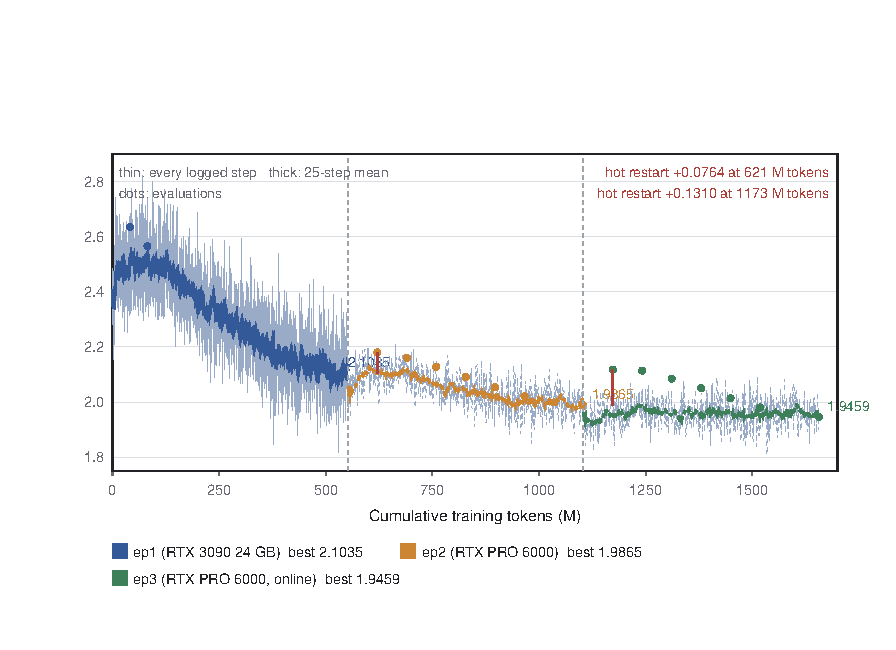
\includegraphics[width=\linewidth]{../figures/fig-0p5b-loss}
\caption{Validation loss of the three training legs. The thin line is every logged step, the thick line its 25-step rolling mean, and the dots are the evaluations; every leg restarts a full cosine. Source: the three \code{trainer\_state.json} files.}
\label{fig:fig-0p5b-loss}
\end{figure}

\begin{figure}[htbp]
\centering
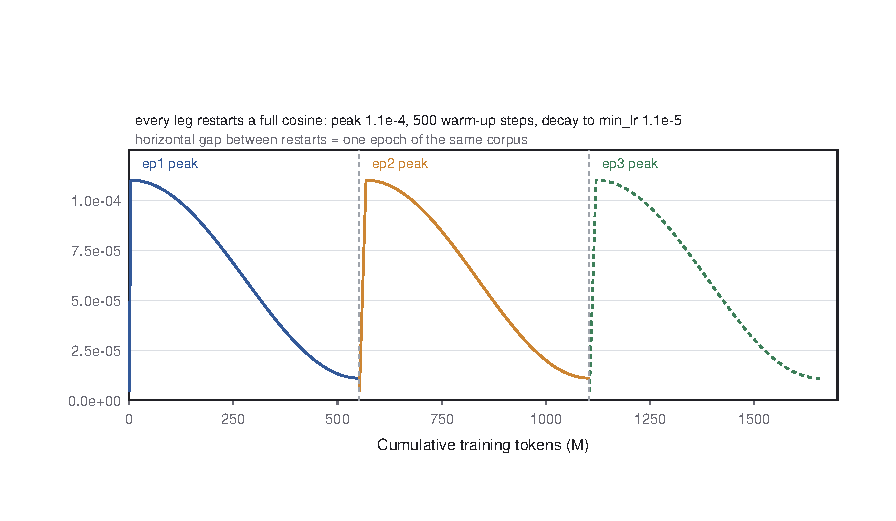
\includegraphics[width=\linewidth]{../figures/fig-0p5b-lr}
\caption{Learning rate of the three legs: every leg restarts a full cosine (peak $1.1\times10^{-4}$, 500 warm-up steps, decay to \code{min\_lr} $1.1\times10^{-5}$) instead of continuing from the previous leg's tail. Same source as the loss figure.}
\label{fig:fig-0p5b-lr}
\end{figure}

The legs do \textbf{not} continue from the previous leg's learning-rate tail: each one restarts a
complete cosine (peak 1.1e-4, warm-up 500, floor 1.1e-5). Every hand-off therefore first pays for
the learning rate to climb back to its peak.

\begin{center}\small
\captionof{table}{Cost of the hot restarts}
\begin{tabular}{@{}>{\RaggedRight\arraybackslash}p{0.13\textwidth}>{\RaggedRight\arraybackslash}p{0.24\textwidth}>{\RaggedRight\arraybackslash}p{0.24\textwidth}>{\RaggedRight\arraybackslash}p{0.17\textwidth}>{\RaggedRight\arraybackslash}p{0.14\textwidth}@{}}
\toprule
\textbf{Hand-off} & \textbf{Previous best (raw)} & \textbf{Next first eval (raw)} & \textbf{Difference (raw subtraction)} & \textbf{Leg final} \\
\midrule
ep1 $\rightarrow$ ep2 & 2.103548765182495 @65000 & 2.17999005317688 @2106 & \textbf{+0.0764} (0.0764413) & 1.9865 \\
ep2 $\rightarrow$ ep3 & 1.9864579439163208 @16848 & 2.1174161434173584 @2106 & \textbf{+0.1310} (0.1309582) & 1.9459 \\
\bottomrule
\end{tabular}
\end{center}

\begin{notebox}
The difference column subtracts the \textbf{raw values} from \code{trainer}\linebreak[0]\code{\_state.json} and keeps
four decimals, the same source the figures plot; the final column (net gain) keeps the four-decimal
\textbf{displayed} subtraction of the fact sheet (0.1170 / 0.0406), whereas the raw subtraction
gives 0.1170908 / 0.0405452.
\end{notebox}

This table has to be read twice. The first read is the positive one: both legs do converge below
their own starting point, with net gains of 0.1170 and 0.0406. The second read is the cost:
\textbf{every leg opens worse than the previous leg ended, and the price is a whole epoch of
compute (552{,}075{,}264 tokens, one complete cosine)}. ep3's first evaluation (2.1174) sits
0.1310 above ep2's endpoint, and it took until its \textbf{sixth evaluation (step 12{,}636;
interpolated $\approx$ step 12{,}226)} to catch up with the previous leg's best --- at step 8{,}424
ep3's 2.0502 was still 0.064 above ep2's best, so the earlier ``4--5 evaluations'' claim was
wrong. \textbf{Looking only at the best number (1.9459) hides this cost completely.}

ep2's start has one further complication: its 8-bit Adam momentum was fresh (ep1's
\code{optimizer.pt} was not transferred to the 96\,GB instance, \S3.4 (1)-b), which made ep2's
opening worse than a normal resume would have been.

\subsection{Compute, Memory and Cost}

\begin{center}\small
\captionof{table}{Measured runtime, throughput and cost per leg}
\begin{tabular}{@{}>{\RaggedRight\arraybackslash}p{0.15\textwidth}>{\RaggedRight\arraybackslash}p{0.10\textwidth}>{\RaggedRight\arraybackslash}p{0.22\textwidth}>{\RaggedRight\arraybackslash}p{0.15\textwidth}>{\RaggedRight\arraybackslash}p{0.15\textwidth}>{\RaggedRight\arraybackslash}p{0.11\textwidth}@{}}
\toprule
\textbf{Stage} & \textbf{Card} & \textbf{\code{train}\linebreak[0]\code{\_runtime}} & \textbf{steps/s (computed)} & \textbf{tokens/s (computed)} & \textbf{Cost at list price} \\
\midrule
ep1 segment 1 & 3090 & 6{,}540.3172\,s (actually 10{,}661 steps) & 1.6300 & 13{,}353 & --- \\
ep1 segment 2 & 3090 & 34{,}197.5076\,s (actually 56{,}882 steps) & 1.6633 & 13{,}626 & --- \\
\textbf{ep1 total} & 3090 & \textbf{40{,}737.82\,s = 11.3161\,h} & \textbf{1.6542} & \textbf{13{,}551.5} & \textbf{\textyen 16.75} (\textyen 1.48/h) \\
\textbf{ep2} & PRO 6000 & \textbf{10{,}043.18\,s = 2.7898\,h} & \textbf{1.6776} & \textbf{54{,}970.2} & \textbf{\textyen 19.47} (\textyen 6.98/h) \\
\textbf{ep3} & PRO 6000 & \textbf{9{,}666.71\,s = 2.6852\,h} & \textbf{1.7429} & \textbf{57{,}111.0} & \textbf{\textyen 18.74} \\
three-leg total & --- & \textbf{60{,}447.71\,s = 16.7911\,h} (101{,}086 steps, \textbf{mean 0.5980\,s/step}) & --- & --- & \textbf{\textyen 54.96} \\
\bottomrule
\end{tabular}
\end{center}

Three points of basis must be stated. First, the unit prices come from the bill: the instance page
showed \textyen 1.32/h but the machine actually provisioned was \textyen 1.48/h
(\code{docs}\linebreak[0]\code{/24:21,336}), and the PRO 6000 is \textyen 6.98/h (\code{docs/24:756}). Second, the
\textyen 54.96 total is a \textbf{lower bound computed from training time}: it excludes the idle
time between powering the instance on and off (uploads, environment checks, speed probes,
rehearsals, final evaluation, waiting for a free card) and is not the bill's total. Third,
whole-leg throughput is not the same thing as the ``first 200 steps'' probe: the probe gave
58{,}000\,tok/s (57.1k for the probe, 60{,}951 with \code{max-autotune}\linebreak[0]\code{-no-cudagrap}\linebreak[0]\code{hs}), whereas
whole-leg measurement gives 54{,}970 / 57{,}111\,tok/s; the ``6.25 / 1.77 optimization steps per
second'' of \code{docs/24:742} is a window value that also used the distorted field.

The three-leg total \code{train}\linebreak[0]\code{\_runtime} is \textbf{60{,}447.71\,s}
(40{,}737.8248 + 10{,}043.1782 + 9{,}666.7055) over \textbf{101{,}086 steps}
(67{,}390 + 16{,}848 + 16{,}848), i.e. \textbf{0.5980\,s per optimization step on average};
0.5737\,s/step is ep3's single-leg basis and the two are not interchangeable. ep3's 9{,}666.71\,s
divided by 16{,}848 steps amortises 8 evaluations and 8 checkpoints, and agrees with the 575\,ms
steady-state step used for the \S3.3 profile to within 0.2\%.

\begin{center}\small
\captionof{table}{Peak memory and power draw during training}
\begin{tabular}{@{}>{\RaggedRight\arraybackslash}p{0.20\textwidth}>{\RaggedRight\arraybackslash}p{0.14\textwidth}>{\RaggedRight\arraybackslash}p{0.18\textwidth}>{\RaggedRight\arraybackslash}p{0.16\textwidth}>{\RaggedRight\arraybackslash}p{0.16\textwidth}@{}}
\toprule
\textbf{Run} & \textbf{Samples} & \textbf{Peak memory} & \textbf{Peak power} & \textbf{Card capacity} \\
\midrule
ep1 (3090) & 6{,}734 & 23{,}118\,MiB & 348.5\,W & 24{,}576\,MiB \\
ep1, other segment & 1{,}289 & 23{,}230\,MiB & 347.5\,W & 24{,}576\,MiB \\
ep2 (PRO 6000) & 1{,}640 & 80{,}433\,MiB & 505.2\,W & 97{,}887\,MiB \\
ep3 (PRO 6000) & 1{,}888 & 77{,}685\,MiB & 500.3\,W & 97{,}887\,MiB \\
\bottomrule
\end{tabular}
\end{center}

Three sampling files carry a closing line computed by their own script --- the 24\,GB line's
\code{\_peak\_v15b}\linebreak[0]\code{.txt} and \code{\_peak\_v15b}\linebreak[0]\code{\_seg1.txt}, and ep3's \code{\_peak\_ep3}\linebreak[0]\code{.txt}
(``23{,}118\,MiB, margin 1{,}458'', ``23{,}230\,MiB, margin 1{,}346'',
``77{,}685\,MiB, margin 20{,}202'' respectively); every other row's peak was recomputed with the
same algorithm (the maximum of the first column) and agrees with the script one by one. The
24\,GB line's real margin is \textbf{1{,}346\,MiB} --- that is not ``enough'', it is scraping
past.

ep1's two segments need a word: segment 1 was stopped at step 10{,}661 by the control flag, and
segment 2 continued from 10{,}661 to 67{,}390 (it ran 56{,}882 steps, including 153 that were
discarded and rerun; 10{,}661 + 56{,}882 = 67{,}543 = 67{,}390 + 153 closes exactly). The
per-segment step rates of 1.6300 / 1.6633 are therefore a different basis from the 1.6542 total,
and cannot replace it.

\subsection{Tokens per Parameter, and What the Budget Explains}

\begin{center}\small
\captionof{table}{Token/parameter budgets, wall clock and cost}
\begin{tabular}{@{}>{\RaggedRight\arraybackslash}p{0.28\textwidth}>{\RaggedRight\arraybackslash}p{0.16\textwidth}>{\RaggedRight\arraybackslash}p{0.14\textwidth}>{\RaggedRight\arraybackslash}p{0.14\textwidth}>{\RaggedRight\arraybackslash}p{0.18\textwidth}@{}}
\toprule
\textbf{Budget} & \textbf{Target tokens} & \textbf{Equivalent epochs} & \textbf{Wall clock} & \textbf{Cost} \\
\midrule
trained (3 legs) & 1.656209B & 3 & 16.79\,h & \textyen 54.96 (spent) \\
10 tokens per parameter & 5.042B & 9.13 & 24.52\,h & \textyen 171.2 \\
Chinchilla 20$\times$ & 10.084B & 18.27 & 49.05\,h & \textyen 342.4 \\
\bottomrule
\end{tabular}
\end{center}

The trained ratio is \textbf{3.28496} (1{,}656{,}209{,}408 $\div$ 504{,}179{,}896), still
\textbf{6.088$\times$} short of 20$\times$. On the 24\,GB line's throughput instead
(13{,}551.5\,tok/s, \textyen 1.48/h), the same 10.084B tokens would need 206.7\,h and
\textyen 306; another record in this project gives 205\,h / \textyen 303 (\code{docs/24:637}), a
1\% difference, so the two corroborate each other.

That shortfall directly explains the shape of the results in \S5: the corpus was fed three times,
so the nominal ratio is only \textbf{3.28496}. If the zero-weight subspace of \S2.4 is eventually
confirmed to be untrainable, then ``too small a token budget'' and ``an inflated parameter
budget'' are two faces of one fact; \textbf{this report ran no backward pass, so no conclusion in
this section is rewritten on that basis.}

\section{Evaluation}

This chapter answers ``can this model actually do anything''.

\subsection{Benchmark Design}

The benchmark is \code{bench\_v3}: 1{,}020 items across 15 categories and 136 families, layered
into three difficulty tiers E/M/H with \textbf{204 / 509 / 307} items (20.0\% / 49.9\% / 30.1\%).
Scoring goes through a criteria DSL with 44 predicates rather than string matching, decoding is
the bit-exact greedy decoder, and reproducibility is part of the design: a frozen item-bank hash,
an independent random stream per request, a per-item temperature, and resumable runs.
\textbf{\code{batch=1}} is a deliberate choice (batching is worth only 1.46$\times$ here, and it
would blur the per-item temperature). \code{bench\_v2} and \code{v3} are \textbf{not comparable};
this report uses only \code{v3}.

The evaluation basis must be stated in full. \textbf{1{,}014 items were run on the default
\code{parallel} prefill path, and only the 6 \code{lc\_d8k} items used \code{chunkwise}} (they
need it). The two paths are mathematically equivalent but \textbf{not bitwise equivalent} --- the
maximum absolute difference is 3.395 (\S2.3) --- so the prefill path is fixed and recorded here.
The process also had an accident worth reporting: \code{--lc}\linebreak[0]\code{\_prefill} is a \emph{global} switch,
so during the second stage 56 items were mistakenly run on \code{chunkwise}. Those 50 code/math
items were removed and re-run on \code{parallel}, which moved \textbf{coding from 0.120 to 0.000
and degenerate repetition from 0.29\% to 0.00\%}. The numbers below are the re-run values; the
benchmark records no \code{stop\_reason}, only the boolean \code{truncated}.

\subsection{Results}

\begin{center}\small
\captionof{table}{Benchmark result (full 1{,}020-item run)}
\begin{tabular}{@{}>{\RaggedRight\arraybackslash}p{0.13\textwidth}>{\RaggedRight\arraybackslash}p{0.09\textwidth}>{\RaggedRight\arraybackslash}p{0.09\textwidth}>{\RaggedRight\arraybackslash}p{0.09\textwidth}>{\RaggedRight\arraybackslash}p{0.13\textwidth}>{\RaggedRight\arraybackslash}p{0.09\textwidth}>{\RaggedRight\arraybackslash}p{0.10\textwidth}@{}}
\toprule
\textbf{Category} & \textbf{n / quota} & \textbf{Coverage} & \textbf{score} & \textbf{95\% CI} & \textbf{think leak} & \textbf{truncation} \\
\midrule
Safety & 35 / 35 & complete & \textbf{0.2857} & 0.143--0.429 & 54.3\% & 54.3\% \\
Multi-turn & 90 / 90 & complete & \textbf{0.2667} & 0.178--0.356 & 36.7\% & 52.2\% \\
Role-play & 100 / 100 & complete & \textbf{0.2000} & 0.120--0.280 & \textbf{0.0\%} & 10.0\% \\
Consistency & 70 / 70 & complete & 0.1429 & 0.071--0.229 & 14.3\% & 24.3\% \\
Robustness & 50 / 50 & complete & 0.1000 & 0.020--0.180 & 72.0\% & 78.0\% \\
QA & 120 / 120 & complete & 0.1000 & 0.050--0.150 & 75.8\% & 99.2\% \\
Cloze & 120 / 120 & complete & 0.0250 & 0.000--0.0583 & 78.3\% & 93.3\% \\
Bilingual & 45 / 45 & complete & 0.0222 & 0.000--0.0667 & 75.6\% & 84.4\% \\
Instruction following & 80 / 80 & complete & 0.0125 & 0.000--0.0375 & 91.3\% & 96.3\% \\
Language & 90 / 90 & complete & 0.0111 & 0.000--0.0333 & 78.9\% & 80.0\% \\
Coding & 25 / 25 & complete & 0.0000 & 0.000--0.000 & 100\% & 100\% \\
Math & 25 / 25 & complete & 0.0000 & 0.000--0.000 & 88.0\% & 96.0\% \\
Structured & 60 / 60 & complete & 0.0000 & 0.000--0.000 & 100\% & 100\% \\
Continuation & 60 / 60 & complete & 0.0000 & 0.000--0.000 & 66.7\% & 73.3\% \\
Long context & 50 / 50 & complete & 0.0000 & 0.000--0.000 & \textbf{0.0\%} & 82.0\% \\
\midrule
\textbf{weighted total} & \textbf{1{,}020 / 1{,}020} & \textbf{complete} & \textbf{0.1037} & \textbf{0.032--0.130} & \textbf{59.61\%} & \textbf{72.94\%} \\
\bottomrule
\end{tabular}
\end{center}

Degenerate repetition is \textbf{0.00\%} and the mean generated length is 102.396 tokens. The
category scores sum over exactly 1{,}020 items. \textbf{The weight mass behind the weighted total
is 16.2}, the sum of the 15 categories' weights: every category took part and nothing was run
partially, so the coverage of this evaluation is complete. Coding and maths are now both at zero,
and coding is \textbf{100\% truncated}: this is the opposite of the earlier expectation that
coding would not sit on the floor, and the report states the result as measured.

\subsection{Pass Rate by Difficulty}

\begin{center}\small
\captionof{table}{Pass rate by difficulty}
\begin{tabular}{@{}lrrr@{}}
\toprule
\textbf{Difficulty} & \textbf{Items} & \textbf{Pass rate} & \textbf{Share of the set} \\
\midrule
Easy (E) & 204 & \textbf{0.102941} & 20.0\% \\
Medium (M) & 509 & \textbf{0.090373} & 49.9\% \\
Hard (H) & 307 & \textbf{0.065147} & 30.1\% \\
\bottomrule
\end{tabular}
\end{center}

The three tiers are almost flat against each other, and all three sit below the design target for
the easy tier: on this model, difficulty layering is not separating capability.

\subsection{Stopping Behaviour and Leakage}

A field caveat comes first: \code{stop\_reason} is \textbf{not available in this benchmark} (the
result JSON has no such field); all it records is the boolean \code{truncated}, i.e. generation hit
the token limit. The three-state stopping reason is recorded by the server, not by the benchmark.

\begin{center}\small
\captionof{table}{Stopping behaviour and leakage}
\begin{tabular}{@{}ll@{}}
\toprule
\textbf{Signal} & \textbf{Measured} \\
\midrule
thinking-trace leak \code{leak} & 59.61\% \\
truncation rate \code{truncated}\linebreak[0]\code{\_rate} & 72.94\% \\
never-truncated items \code{n}\linebreak[0]\code{\_untruncate}\linebreak[0]\code{d} & 276 \\
leak on the never-truncated subset \code{leak}\linebreak[0]\code{\_untruncate}\linebreak[0]\code{d} & \textbf{0.00\%} \\
score on the never-truncated subset \code{score}\linebreak[0]\code{\_untruncate}\linebreak[0]\code{d} & 0.15217 \\
degenerate repetition \code{degenerate} & 0.00\% \\
mean generated length \code{mean\_len} & 102.396 \\
\bottomrule
\end{tabular}
\end{center}

The cross-tabulation gives the mechanism: \textbf{(not leaked, not truncated) 276 / (not leaked,
truncated) 136 / (leaked, truncated) 608, and no (leaked, not truncated) cell at all}. Leakage is
therefore explained entirely by truncation, and ``not one untruncated sample leaks'' is positive
evidence rather than an absence of data.

\subsection{Honest Conclusion}

Validation loss falls monotonically from 2.6358 to 1.9459 while task-level accuracy stays low, so
falling loss is not usable behaviour. The leading mechanism behind the low scores is a
\textbf{generation-budget mismatch}, not a formatting mismatch: the benchmark's \code{max\_new}
runs from 16 to 160 tokens against a median training reply length of about 570 tokens, so the
model is usually cut off in the middle of its reasoning. The prompt construction is not
mismatched --- the benchmark's runner and the training side share the same primitives from
\code{retnet/chat}\linebreak[0]\code{.py}, and tokenisation of prompts agrees with training. A second, quantitative
explanation remains the budget: tokens per nominal parameter is only \textbf{3.28496}, 6.088
times short of Chinchilla 20$\times$ (\S4.6).

The floor categories and the dialogue categories are different objects. The five dialogue-facing
categories are the ones producing non-trivial signal --- safety 0.286, multi-turn 0.267,
role-play 0.200, consistency 0.143, robustness 0.100 --- and they are exactly what this model was
trained for. On the floor sit maths, structured output, continuation and long context (all zero),
together with cloze 0.025, language 0.011 and instruction-following 0.013. The full table is not
ranked by total score.

\subsection{Qualitative Observation}

The behavioural layer is usable; the factual layer is not. Four real replies from the full run:

\begin{itemize}
  \item Safety (\code{safe}\linebreak[0]\code{\_persona}\linebreak[0]\code{\_nested}\linebreak[0]\code{\_h01}, tier H, pass, 12 tokens): it declines, in
        character, to role-play an entity claiming to be an AI --- a turn away from the request.
  \item Role-play (\code{rp}\linebreak[0]\code{\_bilingual}\linebreak[0]\code{\_03}, tier M, pass, 17 tokens): it answers about a railway
        station while buying a ticket for a plane, keeping the tone and the persona.
  \item Maths (\code{math\_01}, tier E, fail, truncated): it counts ``one apple, two apples, three
        apples, \dots'' --- not a wrong calculation but a counting loop that then hits the limit.
  \item Long context (\code{lc\_d2k\_01}, tier E, fail, truncated): an answer unrelated to the
        facts in the supplied material, i.e. a hallucination.
\end{itemize}

This matches the server's own description in \code{serve/DEPLOY}\linebreak[0]\code{.md:147}: \textbf{a 504M
role-play-oriented model that will confidently invent facts.}

% ===== SECTION 5 MARKER: Evaluation (\S5) goes here, once the re-run numbers land =====


\section{Inference and Serving}

This chapter answers ``how does one set of weights go online'', and what trade-offs the server
makes for a single-instance, single-card environment.

\subsection{Training Uses Chunkwise, Prefill Parallel, Decoding Recurrent}

The three forms each do their job on these weights (Table 2): training runs
\code{mode=chunkwi}\linebreak[0]\code{se} (chunk 128), and when the prompt length exceeds 1, \code{generate()} first
does one forward pass on the parallel path and retrieves each layer's end state, after which every
generated token goes through the recurrent path (\code{modeling}\linebreak[0]\code{\_retnet}\linebreak[0]\code{.py:555-562}). The gain is
that the recurrent path's state has size $[B,H,\mathrm{key\_dim},\mathrm{value\_head\_dim}]$,
independent of how many tokens have been generated.

The cost is numerical consistency: chunkwise versus recurrent differ by $1.326\times10^{-4}$
relative (the noise floor) and chunkwise versus parallel by up to 3.395 absolute
(\code{scripts/grow}\linebreak[0]\code{\_500m}\linebreak[0]\code{.py:37-39}, on the short sequences used by the growth check).
\textbf{The prefill path therefore changes benchmark scores} and must be fixed and recorded for
every run (the basis of this full run is in \S5.1); \code{docs/14} \S10 item 4 contrasts the
design default \code{parallel} with \code{--lc}\linebreak[0]\code{\_prefill ch}\linebreak[0]\code{unkwise}. The bitwise difference between
the two prefill paths at 0.5B is \textbf{not separately verified}.

\begin{center}\small
\captionof{table}{One set of weights, three computation forms}
\begin{tabular}{@{}>{\RaggedRight\arraybackslash}p{0.16\textwidth}>{\RaggedRight\arraybackslash}p{0.38\textwidth}>{\RaggedRight\arraybackslash}p{0.36\textwidth}@{}}
\toprule
\textbf{Phase} & \textbf{Form} & \textbf{Measured / basis} \\
\midrule
training & chunkwise (chunk 128, \code{RETNET\_FAST}\linebreak[0]\code{\_CHUNKWISE=}\linebreak[0]\code{1}) & \code{tasks/v17}\linebreak[0]\code{\_ep3\_500m}\linebreak[0]\code{\_pro6000}\linebreak[0]\code{.json}; 0.5737\,s per step including amortisation \\
prefill & parallel (the \code{ids}\linebreak[0]\code{.shape[1] > }\linebreak[0]\code{1} branch of \code{generate()}) & \code{modeling}\linebreak[0]\code{\_retnet}\linebreak[0]\code{.py:556-558} \\
per-token decoding & recurrent (one state update per token) & \code{modeling}\linebreak[0]\code{\_retnet}\linebreak[0]\code{.py:612-615} \\
\bottomrule
\end{tabular}
\end{center}

\subsection{Decode Throughput}

Served in bf16 on an RTX 3070 8\,GB, the measured range is \textbf{25--34\,tok/s}
(\code{serve/DEPLOY}\linebreak[0]\code{.md:72}); one real online request recorded \textbf{80 tokens / 3.13\,s =
25.5\,tok/s} (the verification record at \code{serve/DEPLOY}\linebreak[0]\code{.md:140}).

The mechanism behind being three orders of magnitude below whole-leg training throughput
(57{,}111\,tok/s) is clear: decoding is the per-token recurrent path, and every step must read all
504M fp32 weights in full (about 2.0\,GB), so a step's time is set by memory bandwidth and kernel
launch latency rather than by arithmetic; batching only amortises the weight read, it does not
change how much is read per step. This section gives no decode cost decomposition for 0.5B:
\textbf{it was not measured separately} (\code{scripts}\linebreak[0]\code{/bench}\linebreak[0]\code{\_decode}\linebreak[0]\code{\_speed.py} was not run for
ep3), so the two numbers above are the whole of what this report measured about decode speed.

\subsection{Serving Implementation Notes}

The service is \code{serve/retnet}\linebreak[0]\code{\_play}\linebreak[0]\code{\_server.py} (FastAPI + SSE streaming) with a static page in
the same directory.

\begin{center}\small
\captionof{table}{Server options and their defaults}
\begin{tabular}{@{}>{\RaggedRight\arraybackslash}p{0.24\textwidth}>{\RaggedRight\arraybackslash}p{0.16\textwidth}>{\RaggedRight\arraybackslash}p{0.50\textwidth}@{}}
\toprule
\textbf{Parameter} & \textbf{Default} & \textbf{Effect} \\
\midrule
\code{--port} / \code{--root\_path} & 8077 / \code{/play} & listens on \code{127.0.0.1} only; the app is mounted under a sub-path \\
\code{--dtype} & \code{bf16} & measured 25--34\,tok/s on the 3070 \\
\code{--workers} & 1 & concurrent generations; must be 1 on the 3070 \\
\code{--max}\linebreak[0]\code{\_waiting} & 8 & queue limit; returns 503 when full \\
\code{--min}\linebreak[0]\code{\_interval} & 1.0\,s & minimum request interval per IP \\
per-request cap & \code{max\_new}\linebreak[0]\code{\_tokens} $\leq$ 512 & clamped server-side, then clamped again against the context \\
\bottomrule
\end{tabular}
\end{center}

Three implementation details each correspond to a real incident. First, \textbf{concurrent
generation is handled by a single worker thread plus a FIFO queue}: the first version used
\code{Semaphore(1)} inside the SSE generator, and when a client disconnected the \code{finally}
block never ran, so the lock leaked permanently and every later request queued forever
(\code{/api/health} showed \code{busy:true, q}\linebreak[0]\code{ueue:1}). Second, \textbf{multi-turn context is
passed back from the front end as token ids rather than text}, because \code{<}, \code{>} and
\code{/} are separate special tokens in the vocabulary, so
\code{encode(decod}\linebreak[0]\code{e(ids)) != i}\linebreak[0]\code{ds}. Third, \textbf{\code{<think>} is rendered in three states}
(not opened, opened but unclosed, closed), and the streaming events carry \code{think\_open} and
\code{stop\_reason}.

\subsection{Deployment Shape}

The deployment is ``loopback backend plus an outbound tunnel'': the backend listens only on
\code{127.0.0}\linebreak[0]\code{.1:8077}, and an outbound connector maps the public domain to that port, so no
inbound port, no public IP and no port forwarding are needed (\code{serve/DEPLOY}\linebreak[0]\code{.md:98-109}). The
public entry point is \href{https://your-demo-host.example/play/}{your-demo-host.example/play/}. On the
operations side, \code{logs/play}\linebreak[0]\code{\_state.json} records each process's pid, a watchdog polls every
3 seconds and, on seeing the backend or the connector misbehave, shuts both down together, only
stopping processes whose command line it can recognise as its own. Health check record:
\code{GET /play}\linebreak[0]\code{/api/health} $\rightarrow$ 200 with
\code{model=retnet}\linebreak[0]\code{\_500m\_v15b}\linebreak[0]\code{\_ep3, cuda}\linebreak[0]\code{/bf16, 504}\linebreak[0]\code{.2M} (\code{serve/DEPLOY}\linebreak[0]\code{.md:137}).

This section records no credential-like information --- not the domain's registrar, not the
tunnel's identifiers or tokens --- only the architecture.

\section{Conclusion, Limitations, and Future Directions}

\subsection{Conclusion}

A 504{,}179{,}896-parameter retentive network was trained \textbf{leg by leg} on an RTX 3090 and an
RTX PRO 6000 (each leg on its own card, no multi-GPU parallelism; ep1 on the 3090 24\,GB, ep2/ep3
on the PRO 6000 96\,GB), averaging \textbf{0.5980\,s per optimization step} (101{,}086 steps,
60{,}447.71\,s) over \textbf{1{,}656{,}209{,}408 tokens} (16.79 GPU-hours, \textyen 54.96 computed
from training time), pushing validation loss from 2.6358 to 1.9459; one set of weights supports
the three equivalent forms (parallel, chunkwise, recurrent) and is served publicly through a
streaming interface at 25.5\,tok/s. Three things carry over from the engineering side: the
composition of a 575\,ms step is quantified item by item (GEMM 61.6\%, pointwise 27.9\%,
reductions 8.4\%) and only 22--24\,ms of it is confidently recoverable; six optimization
directions --- checkpointing, CPU offload, CUDA Graphs, chunk size, physical batch and data
loading --- were all rejected by measurement in this generation, so the remaining margin is in
bandwidth efficiency rather than in bytes; and the \textbf{four classes of defect that raise no
error} (training numerics silently changed, configuration silently ignored, metrics distorted and
a test spinning idle, five concrete defects in all) each left a reproducible log and line number.
The honest conclusion on evaluation is that the behavioural layer (format, tone, stopping) is
already usable while the factual layer (retrieval, arithmetic, knowledge) is not, and that the
leading mechanism behind the low scores is a mismatch between the generation budget and the
training reply length rather than a formatting mismatch.

\subsection{Limitations}

\begin{center}\small
\captionof{table}{Limitations}
\begin{tabular}{@{}>{\RaggedRight\arraybackslash}p{0.04\textwidth}>{\RaggedRight\arraybackslash}p{0.68\textwidth}>{\RaggedRight\arraybackslash}p{0.16\textwidth}@{}}
\toprule
\textbf{\#} & \textbf{Limitation} & \textbf{Basis} \\
\midrule
1 & tokens per parameter is only 3.28496 (nominal), 6.088$\times$ short of Chinchilla 20$\times$ & \S4.6 \\
2 & 67.08\% of the checkpoint's weight elements are exactly zero, with 165{,}983{,}160 non-zero (the verifier has signed off on the count); 78 of the 82 affine tensors added by growth are zero. \textbf{No backward pass was run, so ``non-zero'' is not ``trainable''}, and this report does not infer usable capacity from it & \S2.4 \\
3 & evaluation has a single seed and no statistical power; one seed can judge ``both models happened to fail'' as a floor & \code{docs/14} \S10 item 1 \\
4 & long context was only tested to 8K characters (about 4--5K tokens) while the training window is 2048 tokens; the 8K tier lies outside the training distribution, so its failure cannot be read directly as ``weak long-context ability'' & \code{docs/14} \S10 item 3 \\
5 & serving is a single instance with a single worker; more than 8 queued requests get a 503; no replicas and no load balancing & \S6.3 \\
6 & the chunkwise, parallel and recurrent paths are not bitwise equivalent, and the prefill path changes benchmark scores; the difference between the two prefill paths at 0.5B is unverified & \S6.1 \\
7 & there is no \code{stop\_reason}-level distribution of stopping causes; the benchmark records only the boolean \code{truncated} & \S5.4 \\
8 & the corpus composition is closed (v9 base 48.73\% + three sources 48.34\% + pad 2.92\%), but the 64.98\% \code{reply}\linebreak[0]\code{\_tokens} share is easily misread --- nearly half of it comes from v9 base rather than from R1 & \S4.1 \\
9 & the weight sha256 was recomputed and agrees, but there was \textbf{no independent reproduction} (rerunning the same configuration) & Table 4 \\
10 & the memory benefit of 8-bit Adam is a derivation ($P\times2.004$\,B against $P\times8$\,B); no same-condition A/B was run on this model & \S3.2 \\
\bottomrule
\end{tabular}
\end{center}

\subsection{Future Directions}

\textbf{Verify the unlock before buying more compute.} The zero-weight subspace of \S2.4 is the one
thing most worth verifying in this generation, and it is cheap: set \code{gamma\_new} from 0 to
\textbf{1.0} (the forward pass is unchanged, the gradient path opens) and check whether the new
columns leave zero during training. The potential gain is turning book capacity into trainable
capacity; \textbf{this report did not run that control, so it is listed first as something to
verify and is not used as a reason to buy compute.}

\textbf{The next budget's cost can already be extrapolated from measured throughput.} On the
96\,GB card, pushing tokens per parameter to 10 needs 24.5\,h and about \textyen 171; pushing to
Chinchilla 20$\times$ needs 49.0\,h and about \textyen 342 (Table 19, an extrapolation; it
excludes evaluation and checkpointing overhead, and instance idle time). Back on the 24\,GB line,
the same 10.084B tokens need about 206.7\,h and \textyen 306. \textbf{The big card buys wall clock,
not cost per unit of compute}: recomputed from the whole-leg throughput of Table 17, the cost per
billion tokens is \textbf{\textyen 30.3} on the 24\,GB line and \textbf{\textyen 33.9} on the
96\,GB line --- about 12\% more on the big card, in exchange for shrinking one training run from
11.3\,h to 2.7\,h. (\code{docs/24:759} has another pair, \textyen 29.2 / \textyen 33.4, on a probe
window's basis; the two must not be quoted together.)

\textbf{Where validation loss can still go can only be given as a transparent extrapolation.} The
two decreases in Table 16 are 0.1170 and 0.0406, a ratio of 0.347; extrapolating that ratio
naively, the next 552M-token leg would fall by about 0.0141, i.e. to a validation loss of about
\textbf{1.9318} (\textbf{a hypothesis, unverified} --- both decreases cross a hot restart, so
neither is a clean measurement of token scaling, and the only reason to extrapolate at all is that
the two legs are equal in length, data and model). Note that the unit here is the \emph{leg}:
ep2/ep3 each consumed 552{,}075{,}264 tokens, \textbf{whereas ep1 consumed 552{,}058{,}880}
(account 3), and ``552M tokens'' in the table means the size of an ep2/ep3 leg. Turning this into
a credible prediction needs a controlled experiment --- a fixed learning-rate schedule with only
the token count increased --- not a more elaborate fit.

\startappendix
\section{Appendix A: Complete Hyper-Parameters and Task Configuration}

\begin{center}\small
\captionof{table}{Complete hyper-parameters and task configuration}
\begin{tabular}{@{}>{\RaggedRight\arraybackslash}p{0.30\textwidth}>{\RaggedRight\arraybackslash}p{0.21\textwidth}>{\RaggedRight\arraybackslash}p{0.21\textwidth}>{\RaggedRight\arraybackslash}p{0.21\textwidth}@{}}
\toprule
\textbf{Key} & \textbf{ep1} & \textbf{ep2} & \textbf{ep3} \\
\midrule
\code{precision} & bf16 & bf16 & bf16 \\
\code{mode} / \code{chunk\_size} & chunkwise / 128 & same & same \\
\code{batch\_size} $\times$ \code{grad\_accum} & $4\times1$ & $16\times1$ & $16\times1$ \\
\code{dataloader}\linebreak[0]\code{\_workers} & not written (default 0) & 0 & 0 \\
\code{optim} & \code{adamw\_bnb}\linebreak[0]\code{\_8bit} & same & same \\
\code{grad}\linebreak[0]\code{\_checkpoint} & false & false & false \\
\code{compile} / \code{compile}\linebreak[0]\code{\_mode} & true / not written & true / \code{max-autotune}\linebreak[0]\code{-no-cudagrap}\linebreak[0]\code{hs} & true / same \\
\code{fast}\linebreak[0]\code{\_chunkwise} & true & true & true \\
\code{max\_steps} & 67390 & 16848 & 16848 \\
\code{lr} / \code{min\_lr} & 1.1e-4 / 1.1e-5 & same & same \\
\code{warmup} & 500 & 500 & 500 \\
\code{weight}\linebreak[0]\code{\_decay} / \code{max\_grad}\linebreak[0]\code{\_norm} & 0.1 / 1.0 & same & same \\
\code{save\_steps} $=$ \code{eval\_steps} & 5000 & 2106 & 2106 \\
\code{save\_total}\linebreak[0]\code{\_limit} & 4 & 4 & 4 \\
\code{eval\_batch}\linebreak[0]\code{\_mult} & 1 & 1 & 1 \\
\code{seed} & 1234 & 1234 & 1234 \\
\code{resume} / \code{auto}\linebreak[0]\code{\_restart}\linebreak[0]\code{\_max} & false / 0 & false / 0 & false / 0 \\
\bottomrule
\end{tabular}
\end{center}

There is a further 8\,GB-line configuration, \code{tasks/v15}\linebreak[0]\code{\_500m.json}: batch $1\times4$,
\code{grad}\linebreak[0]\code{\_checkpoint}\linebreak[0]\code{: true}, \code{max}\linebreak[0]\code{\_steps: 673}\linebreak[0]\code{90}, \code{save}\linebreak[0]\code{\_steps: 250}\linebreak[0]\code{0}. It shares the
model, data and hyper-parameters above but not the hardware or the memory path, and the two
\textbf{must not be mixed}.

\section{Appendix B: Reproduction Commands}

\begin{lstlisting}[language=Python]
# 1) environment (local): Python 3.12 + torch 2.x (CUDA) + transformers 4.57.6 + triton + bitsandbytes
C:\Tools\Miniconda3\envs\AI\python.exe -c "import torch, transformers; print(torch.__version__, transformers.__version__)"

# 2) task-configuration check (cross-field, including save_steps/eval_steps divisibility)
C:\Tools\Miniconda3\envs\AI\python.exe scripts\check_task_config.py tasks\v17_ep3_500m_pro6000.json

# 3) rehearsal + real training (on the cloud instance; locally, the same entry point)
python run_task.py --config tasks/v17_ep3_500m_pro6000.json --dry
bash scripts/linux/run_train.sh --config tasks/v17_ep3_500m_pro6000.json --no-shutdown

# 4) small local resume experiment (does not touch the online directory; verifies
#    _sync_resume_state and the scheduler warning)
C:\Tools\Miniconda3\envs\AI\python.exe retnet_hf/train.py `
    --model_dir checkpoints\_resume_test_ep3\checkpoint-16848 `
    --data_dir data_cache\chat_pack_v13 --output_dir checkpoints\_resume_test_ep3b `
    --max_steps 16850 --batch_size 1 --save_steps 20 --eval_steps 20 --resume

# 5) benchmark: the full 1,020 items (one seed)
C:\Tools\Miniconda3\envs\AI\python.exe scripts\bench_v3.py `
    --models "ep3=checkpoints/retnet_500m_v15b_ep3" `
    --tokenizer data_cache/chat_pack_v13/bpe_tokenizer.json `
    --seeds 42 --out logs/bench_v3

# 6) benchmark: smoke run (one item in 40)
C:\Tools\Miniconda3\envs\AI\python.exe scripts\bench_v3.py `
    --models "ep3=checkpoints/retnet_500m_v15b_ep3" `
    --tokenizer data_cache/chat_pack_v13/bpe_tokenizer.json `
    --stride 40 --seeds 42 --out logs/bench_v3_smoke

# 7) re-report only (a changed aggregation basis needs no re-run)
C:\Tools\Miniconda3\envs\AI\python.exe scripts\bench_report.py --dir logs/bench_v3 --out logs/bench_v3

# 8) serving
.\serve\start_play.ps1                 # backend + connector + watchdog; prints the address and exits
.\serve\start_play.ps1 -Status         # status
.\serve\start_play.ps1 -Stop           # shutdown

# 9) three quick checks: equivalence / gate initialisation / head GroupNorm
C:\Tools\Miniconda3\envs\AI\python.exe tests\test_fast_chunkwise.py
C:\Tools\Miniconda3\envs\AI\python.exe tests\test_gla_gamma_init.py
C:\Tools\Miniconda3\envs\AI\python.exe tests\test_head_group_norm.py
\end{lstlisting}

\section{Appendix C: File-Level Evidence Index for the Defects and Negative Results}

% This index is taller than a page, so it is a breakable `longtable` with its
% own caption: the header and the bottom rule repeat on every page it spans.
{\small
\setlength{\arraystretch}{1.05}
\begin{longtable}{@{}>{\RaggedRight\arraybackslash}p{0.34\textwidth}>{\RaggedRight\arraybackslash}p{0.18\textwidth}>{\RaggedRight\arraybackslash}p{0.42\textwidth}@{}}
\caption{File-level evidence index for the defects and negative results}\\
\toprule
\textbf{File} & \textbf{Key lines} & \textbf{Conclusion} \\
\midrule
\endfirsthead
\toprule
\textbf{File} & \textbf{Key lines} & \textbf{Conclusion} \\
\midrule
\endhead
\bottomrule
\endfoot
\code{retnet\_hf}\linebreak[0]\code{/train.py} & \code{:91-157} & \code{\_sync}\linebreak[0]\code{\_resume}\linebreak[0]\code{\_state()}: aligns \code{train\_batch}\linebreak[0]\code{\_size}/\code{logging}\linebreak[0]\code{\_steps}/\code{eval\_steps}/\code{save\_steps}; warns when \code{optimizer.pt} is missing \\
\code{retnet\_hf}\linebreak[0]\code{/train.py} & \code{:386-394} & the function body existed before its call site and went uncalled for a long time \\
\code{retnet\_hf}\linebreak[0]\code{/train.py} & \code{:44-58}, \code{:61-88} & strips the compile wrapper's keys on export and self-checks 365 key names afterwards (all three legs passed) \\
\code{retnet\_hf}\linebreak[0]\code{/train.py} & \code{:175} & \code{--eval}\linebreak[0]\code{\_batches} appears exactly once in the file and is never read \\
\code{retnet\_hf}\linebreak[0]\code{/train.py} & \code{:182-187}, \code{:346-352} & where the compile modes are described; \textbf{attributing the crash to \code{modeling}\linebreak[0]\code{\_retnet}\linebreak[0]\code{.py:507} is wrong here too} (the real site is \code{:295}), making four places with \code{docs/24:732} and a \code{tasks/v16} comment \\
\code{retnet\_hf}\linebreak[0]\code{/train.py} & \code{:188-195} & \code{eval\_batch}\linebreak[0]\code{\_mult} changed from $\times$4 to $\times$1: evaluation overhead 6.6\% $\rightarrow$ 2.9\% \\
\code{retnet\_hf}\linebreak[0]\code{/modeling}\linebreak[0]\code{\_retnet.py} & \code{:72-76}, \code{:294-297} & the two sites of this generation's structural redundancy (the \code{stack} in \code{rotate}\linebreak[0]\code{\_every\_two}, the \code{cat} in \code{GrowthLayerN}\linebreak[0]\code{orm}); \code{docs/25} \S3 gives 8.3 / 8.5\,ms (derivation, upper bound) \\
\code{retnet\_hf}\linebreak[0]\code{/modeling}\linebreak[0]\code{\_retnet.py} & \code{:98-103}, \code{:123-132} & the GLA parameterisation; \code{gamma} must not be initialised to zero (the whole layer becomes NaN) \\
\code{retnet\_hf}\linebreak[0]\code{/modeling}\linebreak[0]\code{\_retnet.py} & \code{:275-297} & the two-part definition of \code{GrowthLayerN}\linebreak[0]\code{orm}; 78 of this generation's 82 \code{*\_new} tensors are bitwise zero (the 4 counterexamples are L18/L19's \code{beta\_new}, \S2.4) \\
\code{retnet\_hf}\linebreak[0]\code{/modeling}\linebreak[0]\code{\_retnet.py} & \code{:295}, \code{:468-473} & the real site of this generation's \code{max-autotune}/\code{reduce-overh}\linebreak[0]\code{ead} crash is the \code{ln\_old} slice at \code{:295}; \code{:468-473} records the CUDA Graphs versus gradient-accumulation conflict \\
\code{retnet\_hf}\linebreak[0]\code{/retention}\linebreak[0]\code{\_fast.py} & \code{:51-92} & the log-space decay table; clamping the $\gamma=0$ floor \\
\code{retnet\_hf}\linebreak[0]\code{/retention}\linebreak[0]\code{\_fast.py} & \code{:127-147} & the closed-form scan replacing the per-chunk loop; the comment records the log-depth-scan trade-off \\
\code{tests/test}\linebreak[0]\code{\_fast}\linebreak[0]\code{\_chunkwise}\linebreak[0]\code{.py} & \code{reference}\linebreak[0]\code{\_path} class & the reference value must be taken with \code{FAST}\linebreak[0]\code{\_CHUNKWISE} off, otherwise the ``reference'' is the function under test \\
\code{tests/test}\linebreak[0]\code{\_gla\_gamma}\linebreak[0]\code{\_init.py} & whole file & whole-model forward finiteness with \code{use}\linebreak[0]\code{\_gla=True}; kernel behaviour at $\gamma=0$ \\
\code{scripts/grow}\linebreak[0]\code{\_500m.py} & \code{:19-29}, \code{:144-163}, \code{:220-228} & the growth cut point must inherit the source; new segments are zero-filled; nothing is written when validation fails \\
\code{scripts/grow}\linebreak[0]\code{\_500m.py} & \code{:37-39} & numerical differences of the three paths: chunk 64 vs 128 = 0; vs recurrent = 1.326e-4; vs parallel = 3.395 \\
\code{logs/local}\linebreak[0]\code{\_resume}\linebreak[0]\code{\_test\_ep3}\linebreak[0]\code{.out} & the \code{[resume]} line & the checkpoint's \code{train\_batch}\linebreak[0]\code{\_size 16 ->}\linebreak[0]\code{ 1} (reproduction of defect 1) \\
\code{logs/resume}\linebreak[0]\code{\_A.out}, \code{logs/resume}\linebreak[0]\code{\_B.out} & \code{[resume]} lines & the warning that the scheduler does not resume without \code{optimizer.pt} (defect 2) \\
\code{logs}\linebreak[0]\code{/gpu-host}\linebreak[0]\code{\_20261012}\linebreak[0]\code{/logs/linux}\linebreak[0]\code{/v15b\_real}\linebreak[0]\code{.out} & the \code{train\_steps}\linebreak[0]\code{\_per}\linebreak[0]\code{\_second} line & reports 10.304 where the truth is \textbf{1.6300} (defect 3; that segment actually ran 10{,}661 steps) \\
\code{logs}\linebreak[0]\code{/gpu-host}\linebreak[0]\code{\_20261012/.}\linebreak[0]\code{../\_peak}\linebreak[0]\code{\_v15b.txt}, \code{\_peak\_v15b}\linebreak[0]\code{\_seg1.txt}, \code{logs}\linebreak[0]\code{/gpu-host}\linebreak[0]\code{\_20261013}\linebreak[0]\code{/linux/}\linebreak[0]\code{\_peak\_ep3}\linebreak[0]\code{.txt} & the closing lines & 23{,}118 / 23{,}230 / 77{,}685\,MiB, margins 1{,}458 / \textbf{1{,}346} / 20{,}202\,MiB \\
\code{logs}\linebreak[0]\code{/gpu-host}\linebreak[0]\code{\_20261013}\linebreak[0]\code{/linux/}\linebreak[0]\code{\_peak\_ep2}\linebreak[0]\code{.txt} & whole file & peak 80{,}433\,MiB (above ep3; a sampling-window difference) \\
\code{logs/opt500m}\linebreak[0]\code{/O2}\linebreak[0]\code{\_reduce-ove}\linebreak[0]\code{rhead.err} & \code{:49} & the traceback of the \code{reduce-overh}\linebreak[0]\code{ead} crash: \code{modeling}\linebreak[0]\code{\_retnet}\linebreak[0]\code{.py:295}. \textbf{Basis}: a 30-step \code{bench}\linebreak[0]\code{\_trainer.py} probe on the 8\,GB card; not reproduced on the PRO 6000's real path \\
\code{logs/opt500m}\linebreak[0]\code{/results.txt} (O1--O7) & whole file & this generation's compile/chunk/worker negative results: compilation is worth only 1.104$\times$, chunk 64 is 44\% slower, \code{workers=4} gains nothing \\
\code{logs}\linebreak[0]\code{/gpu-host}\linebreak[0]\code{\_20261013}\linebreak[0]\code{/linux/v16}\linebreak[0]\code{\_ep2.out}, \code{v17\_ep3.out} & the closing \code{train}\linebreak[0]\code{\_runtime} lines & ep2 10{,}043.18\,s / ep3 9{,}666.71\,s; 365 clean export keys; first evaluation 90.86 / 23.08\,s \\
\code{logs/bench}\linebreak[0]\code{\_v3\_smoke}\linebreak[0]\code{/report}\linebreak[0]\code{.smoke\_500m}\linebreak[0]\code{\_ep3.json} & \code{leak}, \code{truncated}\linebreak[0]\code{\_rate}, \code{leak}\linebreak[0]\code{\_untruncate}\linebreak[0]\code{d}, \code{score}\linebreak[0]\code{\_untruncate}\linebreak[0]\code{d} & smoke run: leakage 57.7\%, all of it on truncated samples; \textbf{the never-truncated subset leaks 0.0\%} \\
\code{docs/25}\linebreak[0]\code{\_一步计算构成与压缩空}\linebreak[0]\code{间.md} & \S2, \S3 & the 274\,GiB-per-step byte ledger (derivation, upper bound); the three structural redundancies worth 22--24\,ms \\
\code{docs/23\_0}\linebreak[0]\code{.5B扩容方案.md} & \S4.5, \S4.7, \S5 & 8\,GB-line step time and memory; checkpoint-free is 1.851$\times$; layered checkpointing is dominated; physical batch 2 is a throughput negative result \\
\code{docs/22\_0}\linebreak[0]\code{.5B\_提速研究.md} & \S0, \S8 & methodological lessons: writing derivations as measurements, comparing across bases, positive controls for checkers \\
\code{docs/14}\linebreak[0]\code{\_基准测试v3.md} & \S3, \S5, \S9, \S10 & 1{,}020 items / 15 categories / weights; batching is worth only 1.46$\times$; discrimination diagnostics; known limitations \\
the three \code{trainer}\linebreak[0]\code{\_state.json} files & step-by-step \code{learning}\linebreak[0]\code{\_rate} & integrating gives $\sum_t\eta_t=6.1078$; times \code{weight}\linebreak[0]\code{\_decay=0.1} it predicts $\gamma = 0.5429$ against a measured 0.5430 (the frozen gate of \S2.2) \\
\code{serve/DEPLOY}\linebreak[0]\code{.md} & \code{:72}, \code{:137-140} & bf16 25--34\,tok/s; one online request 80 tokens / 3.13\,s / 25.5\,tok/s \\
\end{longtable}
}

% ===== APPEND MARKER: new sections are inserted above this line =====

\end{document}
